% -----------------------------------------  
% Autogenerated LaTeX file from XML DocBook  
% -----------------------------------------  
%%<params>
%% document.language en
%%</params>
\documentclass{report}
\IfFileExists{ifxetex.sty}{%
    \usepackage{ifxetex}%
  }{%
    \newif\ifxetex
    \xetexfalse
  }
  \ifxetex
\usepackage{fontspec}
\usepackage{xltxtra}
\defaultfontfeatures{Mapping=tex-text}
\setmainfont{DejaVu Serif}
\setsansfont{DejaVu Sans}
\setmonofont{DejaVu Sans Mono}
\else
\usepackage[T1]{fontenc}
\usepackage[latin1]{inputenc}
\fi
\usepackage{fancybox}
\usepackage{makeidx}
\usepackage[hyperlink]{docbook}
\renewcommand{\DBKreleaseinfo}{}
\setcounter{tocdepth}{5}
\setcounter{secnumdepth}{5}


\def\DBKsubtitle{from startup to enterprise (Student Edition)}

\renewcommand{\DBKdate}{2016-{}11-{}26}



\title{The digital professional}
\author{Charles T. Betz}
\hypersetup{%
pdfcreator={DBLaTeX-0.3.7},%
pdftitle={The digital professional},%
pdfauthor={Charles T. Betz}}
% ------------------
% Collaborators
% ------------------
\renewcommand{\DBKindexation}{
\begin{DBKindtable}
\DBKinditem{\writtenby}{Charles T. Betz}
\end{DBKindtable}
}
\makeindex
\makeglossary
\begin{document}
\lstsetup
\frontmatter
\maketitle
\tableofcontents
\listoffigures
\mainmatter

% ------- 
% Chapter 
% ------- 

\chapter{Praise for this book}
\label{Praise}\hyperlabel{Praise}%
  
\emph{Agile IT Management is a perfect fit for my Management Information Systems class to introduce students to the fast-{}paced world of IT Infrastructure that they will be dealing with shortly upon graduation.  This book uses multiple perspectives (Founder, Team Leader, VP, C-{}level executive) to demonstrate to the student not only how a business grows, but how they need to continually grow their skill set.  The use of hands-{}on exercises encouraged by the format of this book complements my teaching style that allows students to learn by doing, failing and doing again.  An additional benefit is that this book begins with a focus on the startup mentality which I will use in my Business Innovation class.}
 
\emph{Prof. Pat Paulson, Winona State University}
 
% ------- 
% Chapter 
% ------- 

\chapter{Copyright}
\label{Copyright}\hyperlabel{Copyright}%
  
The digital professional: From startup to enterprise
 
Published by Digital Management Academy, LLC 14 Sidney Place Minneapolis, MN  55414
 
Copyright � 2016 by Charles T. Betz
 
All rights reserved, for information about permission to reproduce selections from this book, write to Permissions, Digital Management Academy LLC,
14 Sidney Place, Minneapolis, MN  55414
 
First Edition
 
Produced in the United States of America
 
Cover illustration by Go To Media, LLC
 
ISBN: 978-{}0-{}9981346-{}0-{}4
 
Publisher's note to readers:
Although the author and publisher have made every effort to ensure that the information in this book was correct at press time, the author and publisher do not assume and hereby disclaim any liability to any party for any loss, damage, or disruption caused by errors or omissions, whether such errors or omissions result from negligence, accident, or any other cause.
 
For information about special discounts for bulk purchases or for information on booking authors for an event, please visit www.dm-{}academy.com.
 
% ------- 
% Chapter 
% ------- 

\chapter{Dedication}
\label{Dedication}\hyperlabel{Dedication}%
  
\emph{To my students}
 
% ------- 
% Chapter 
% ------- 

\chapter{Preface}
\label{Preface}\hyperlabel{Preface}%
  
In 2013, I was approached by Dr. Bhabani Misra, the head of the Graduate Programs in Software at the University of St. Thomas in St. Paul. Dr. Misra asked me to teach an "IT Infrastructure" course (SEIS660), focusing on the Information Technology Infrastructure Library, or ITIL.
 
The first semester of the class was well received enough for me to be invited back. However, there were complaints from the students that it was too "theoretical." I was attempting to teach using an enterprise architecture style, with lots of abstractions, that just was not engaging students effectively.
 
I also had a team project approach that immediately started the students out as the IT leadership team of a large corporation. This generated feedback that the students wanted something more practical; they were not going to be immediately hired as senior executives!
 
I took this feedback seriously. I especially gave thought to a practical aspect, and so started to develop a lab component. This was and is popular with the students. I also started to think about different approaches for structuring the class that would make more sense for a survey class with a wide spectrum of experience.
 
For three semesters I assigned my first book (\emph{Architecture and Patterns for IT: Service Management, Resource Planning, and Governance}) as a required text for the class. However, I did not write this as a textbook and its limitations became clearer and clearer. It has a strongly architectural approach, approaching the IT management problem as a series of \href{https://en.wikipedia.org/wiki/4%2B1_architectural_view_model}{views on a model}. I do not recommend this as a pedagogical approach for a survey class.
 
I approached my publisher with the idea of a 3rd edition that would pivot the existing material towards being something more useful in class. They agreed to this and I started the rewrite.
 
However, by the time I was halfway done with the first draft, I had a completely new book. Material from the previous work simply did not fit the emergence model used to structure the narrative.
 
A number of factors converged at this point:
 \begin{itemize}

\item{} My view that the "medium is the message" and this extends to choice of authoring approach, intellectual property, DRM, and publisher
 

\item{} Contacts with local and international faculty and thought leaders, and a desire to openly collaborate with them on making the book as good as possible
 

\item{} A desire to freely share at least a rough version of the book, both for marketing purposes and in the interests of giving back to the global IT community
 

\item{} A desire to be able to rapidly update the book with as little friction as possible
 

\item{} A practical realization that the book might get more uptake globally if available at least in some form as free and open source IP
 

\item{} The fact I had already started to \href{https://github.com/StThomas-SEIS660}{publish my labs on Github}, and had in fact had developed a workable continuous delivery ("DevOps") toolchain (the \href{https://github.com/CharlesTBetz/Calavera}{Calavera project}, which has attracted collaborators from the US, Spain, and Israel).
 
\end{itemize}
 
Many have assisted with this work:
 
Thanks to Dr. Bhabani Misra for asking me to teach at the University of St. Thomas and providing direction at key points.
 
Thanks to Stephen Fralippolippi and Roger K. Williams for being the first Github contributors.
 
Thanks to Jason Baker for text and technical collaboration.
 
Thanks to Mark Kennaley for guidance on open versus closed loop thinking.
 
Thanks to Glen Alleman for guidance on modern project management practices.
 
Thanks to Jeff Sussna for ongoing inspiration, Twitter feedback, discussion question ideas, and sourced quotes.
 
Thanks to Nicole Forsgren for links to articles on performance management.
 
Thanks to Evan Leybourn for detailed commentary on project management/Chapter 8.
 
Thanks to Chris Little and Jabe Bloom for quote provenance.
 
Thanks to Lorin Hochstein for references.
 
Thanks to Gene Kim for ongoing mentoring and advice on writing and publishing, and unwavering support and confidence in my efforts.
 
Thanks to the Go to Marketing team (Will Goddard, Terry Brown, Francisco Piniero) for design assistance and invaluable partnership.
 
Thanks to Professor Pat Paulson for being the first adopter of the textbook, and thanks to his students for invaluable criticism and feedback.
 
% ------- 
% Chapter 
% ------- 

\chapter{Introduction}
\label{Introduction}\hyperlabel{Introduction}%
  
\section{For the student}
\label{_for_the_student}\hyperlabel{_for_the_student}%
  
This is a "survey" text intended for the advanced undergraduate or graduate student interested in the general field of applied IT management. It is grounded in basic computing fundamentals, but does not require any particular technical skills to understand. You do not need to have taken any courses in networking, security, or particular programming languages to read this book.
 
However, you will be presented with material on such topics, including fragments of programming languages and pseudocode, and need to be willing to invest the time and effort to understand.
 
This book makes frequent reference to digital startups -{} early stage companies bringing new  products to market that are primarily delivered as some form of computer-{}based service. Whether or not you intend to pursue such endeavors, the startup journey is a powerful one for your learning. Large information technology organizations in enterprises sometimes gain a reputation for losing sight of business value. IT seems to be acquired and operated for its own sake. Statements like "we need to align IT with the business!" are too often heard.
 
A digital startup exposes with great clarity the linkage between "IT" and "the business." The success or failure of the company itself depends on the adept and responsive creation and deployment of the software-{}based systems. Market revenues arrive, or do not, based on digital product strategy and the priorities chosen. Features the market doesn't need? You won't have the money to stay in business. Great features, but your product is unstable and unreliable? Your customers will go to the competition.
 
The lessons that digital entrepreneurs have learned through this trial by fire shed great light on IT's value to the business. Thinking about a startup allows us to consider the most fundamental principles as a sort of microcosm, a small laboratory model of the same problems that the largest enterprises face.
 
However, this is not a textbook (or course) on entrepreneurship. It remains IT-{}centric. \textbf{And, the book is also intended to be relevant to students entering directly into large, established enterprises.} In fact, it prepares the student for working in all stages of growth because it progresses through these four contexts:
 \begin{itemize}

\item{} Individual (founder)
 

\item{} Team
 

\item{} Small company (team of teams)
 

\item{} Enterprise
 
\end{itemize}
 
Whether in a startup, or on a journey within a larger, established organization, you will (hopefully) become aware as you progress through a broadening context:
 \begin{itemize}

\item{} Other team members
 

\item{} Customers
 

\item{} Suppliers
 

\item{} Sponsors
 

\item{} Necessary non-{}IT capabilities (finance, legal, HR, sales, marketing, etc)
 

\item{} Channel partners
 

\item{} Senior executives and funders
 

\item{} Auditors and regulators
 
\end{itemize}
 
Part of maturing in one's career is understanding how all these relationships figure into your own overall system of value delivery. This will be a lifelong journey for the student; the author's intent is to provide some useful tools.
  
\section{Assumptions of the reader}
\label{_assumptions_of_the_reader}\hyperlabel{_assumptions_of_the_reader}%
  \begin{itemize}

\item{} This book is written at the advanced undergraduate/graduate student level. It is currently available only in English.
 

\item{} There is no assumption of deep IT experience, but there is an assumption that the person interacts with computers in some capacity and has basic technical literacy. They should for example understand the concept of an "operating system." An A+ certification, or an intro to programming class for example, would more than adequately prepare someone for this book.
 

\item{} A person completely unfamiliar with computing will need to supplement their reading as suggested throughout the text. There is a wealth of free and accurate information on IT fundamentals (e.g. compute, storage, networking, programming, etc) and this book seeks more to curate than replicate.
 
\end{itemize}
  
\section{This book's structure}
\label{_this_book_s_structure}\hyperlabel{_this_book_s_structure}%
  
Here is a conceptual illustration of an IT management progression (read bottom to top):
 \begin{figure}[H]

\begin{center}
\imgexists{images/ITProgression.png}{{\imgevalsize{images/ITProgression.png}{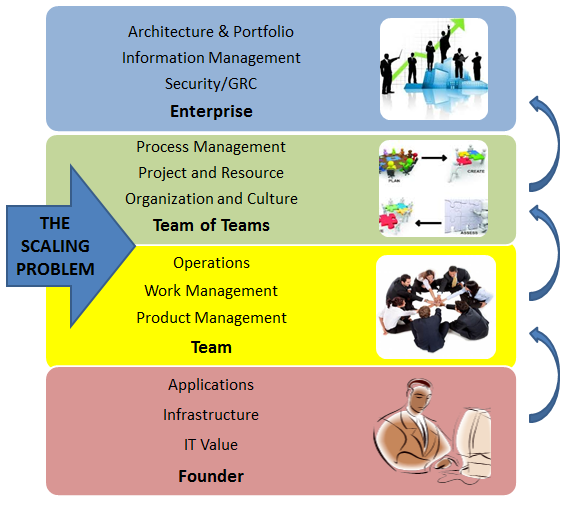
\includegraphics[width=\imgwidth,height=\imgheight,keepaspectratio=true]{images/ITProgression.png}}}}{ITProgression}
\end{center}
\caption{IT management evolutionary model (read bottom to top)}
\end{figure}
 
Elaborating the above outline into chapters, we have:
 \begin{enumerate}[label=\Roman*.]

\item{} \textbf{Founder}
 \begin{enumerate}[label=\arabic*.]

\item{} \emph{IT value}. Why do we need computers? What can they do for us?
 

\item{} \emph{IT infrastructure} We want to build something. We have to choose a platform first.
 

\item{} \emph{IT applications} Let's start building something of use to someone.
 
\end{enumerate}
 

\item{} \textbf{Team}
 \begin{enumerate}[label=\arabic*.]

\item{} \emph{Product management} What exactly is it we are building? What is the process of discovering our customer's needs and quickly testing how to meet them? How do we better define the product vision, and the way of working towards it, for a bigger team?
 

\item{} \emph{Work management} How do we keep track of what we are doing, and communicate our progress and needs at the simplest level?
 

\item{} \emph{Operations management} How do we sustain this surprisingly fragile digital service, in its ongoing delivery of value?
 
\end{enumerate}
 
\end{enumerate}
 
\emph{The boundary between the "team" and the "team of teams" is a challenging area, and industry responses remain incomplete and evolving. Hence the notation "THE SCALING PROBLEM" on the diagram.}
 \begin{enumerate}[label=\Roman*.]

\item{} \textbf{Team of Teams}
 \begin{enumerate}[label=\arabic*.]

\item{} \emph{Organization and culture} We're getting big. How do we deal with this? How are we structured? Why this way and not that? How can we benefit from increasing maturity and specialization, while still maintaining a responsive product? What are the unwritten values and rules in our company?
 

\item{} \emph{Investment, sourcing, and people} Work is becoming larger and more complex. How can we  track and execute larger segments of it, and coordinate across multiple teams?
 

\item{} \emph{Execution management} We have a structure. Work needs to flow across it. Product and project teams increasingly demand predictable, consistent delivery of internal services, and synchronization points such as enterprise releases are increasingly critical signals.
 
\end{enumerate}
 

\item{} \textbf{Enterprise}
 \begin{enumerate}[label=\arabic*.]

\item{} \emph{Governance, risk, security, and compliance} We need to cope with external forces (regulators, vendor partners, security adversaries, auditors) increasingly defining our options.
 

\item{} \emph{Enterprise information management} We've been concerned with data, information, and knowledge since the earliest days of our journey. But at this scale, we have to formalize our approaches and understandings; without that, we will never capture the full value available with modern analytics and Big Data. Compliance issues are also compelling us to formalize here.
 

\item{} \emph{Architecture and portfolio} We need to understand the big picture of interacting lifecycles, reduce technical debt and redundancy, accelerate development through establishing platforms, and obtain better economies of scale. We need to define our investment strategy based on a sound understanding of both business needs and technology limitations.
 
\end{enumerate}
 

\item{} \textbf{Appendices}
 \begin{enumerate}[label=\arabic*.]

\item{} \emph{A review of IT frameworks and standards}
 

\item{} \emph{Architectural depictions}
 

\item{} \emph{Towards a theory of IT management}
 
\end{enumerate}
 
\end{enumerate}
 
The intent is that the more complex, "enterprise"-{}scale concerns at the end of the book are presented as part of a logical progression.
 
\label{formalization}\hyperlabel{formalization}
  
\section{Emergence means formalization}
\label{_emergence_means_formalization}\hyperlabel{_emergence_means_formalization}%
  
The emergence model seeks to define a likely order in which concerns are \textbf{formalized}. Any concern may of course arise at any time: the startup founder certainly is concerned with security!
 
Formalization means at least one or more of the following:
 \begin{itemize}

\item{} Dedicated resources
 

\item{} Dedicated organization
 

\item{} Defined policies and processes
 

\item{} Automated tooling
 
\end{itemize}
 
In the author's experience, for example, startups avoid formalized process and project management. To the extent the concerns exist, they are \emph{tacit} (understood or implied; suggested; implicit). Certainly, a small startup does not invest in an enterprise-{}class service desk tool supporting a full array of IT management processes, or a full-{}blown Project Management Office with its own Vice President and associated portfolio automation. Simple work management, with a manual or automated Kanban board, is likely their choice for work management.
 
But by the time they are a team of teams, specialization has emerged and more robust processes and tools are required. The danger of course is that the formalization effort may be driven by its own logic, and start to lose track of the all-{}critical business context.
 
By careful examining these stages of maturation, and the industry responses to them, it is the author's hope that the student will have effective tools to critically engage with the problem of scaling the digital organization.
  
% ------- 
% Chapter 
% ------- 

\chapter{Part I: Founder}
\label{Part-I-intro}\hyperlabel{Part-I-intro}%
  
\label{Sec-I}\hyperlabel{Sec-I} This is the introduction to Part I.
 
In this section, we  explore the fundamentals of information technology delivery.
 
\textbf{Scenario}
 
You are working in a startup, alone or with one or two partners. You are always in the same room, easily able to carry on a running conversation about your efforts and progress. You have no time or resources to spend on anything except keeping your new system alive and running.
 
\textbf{Chapter 1: IT Value}
 
Chapter 1 introduces you to the fundamental concepts of IT value that serve as a basis for the rest of the course. Why do people want computing (IT) services? What are the general outlines of their structure? How do they come into being? How are they changed over time?
 
All of this is essential to understand for your scenario; you need to understand what computers can do and how they are generally used, if you are going to create a product based on them.
 
This chapter also covers the basics of how you'll approach building a product. It's assumed you won't develop an intricate, long-{}range plan but rather will be experimenting with various ideas and looking for "fast feedback" on their success or failure.
 
\textbf{Chapter 2: IT Infrastructure}
 
In this chapter, you have a general idea for a product and are ready to start building it. But not so fast\ldots{}\hspace{0em} you need to decide some fundamentals first. How will your new product run? What will you use to build it?
 
It's not possible to begin construction until you decide on your tools. This chapter will provide you an overview of computing infrastructure including Cloud hosting and various approaches to system configuration.
 
This chapter also presents an overview of source control, as even your infrastructure depends on it in the new world of "infrastructure as code."
 
\textbf{Chapter 3: Application delivery}
 
Finally, you're ready to start building something. While this is not a book on software development or programming languages, it's important to understand some basics and at least see them in action.
 
This is also the "DevOps" chapter; it's not just about writing code, but about the entire end to end system that gets the code you are writing from your workstation, into collaborative environments, and finally to a state where it can be accessed by end users. From source repository to build manager to package repository to production, we'll cover a basic toolchain that will help you understand modern industrial practices.
 
\textbf{This section's lab approach}
 
While this is not a book about any particular computing language or platform, we need to describe some technical fundamentals. We'll do so in as neutral a manner as possible. However, this books' accompanying labs are based on \href{http://www.ubuntu.com/}{Ubuntu Linux} and \href{https://git-scm.com/}{git}, the distributed version control system created by Linus Torvalds to facilitate Linux development.
 \begin{DBKadmonition}{warning}{Important}
 
Part II, like the other parts, needs to be understood as a unified whole. In reality, digital entrepreneurs struggle with the issues in all three chapters simultaneously.
 \end{DBKadmonition}
 
\section{Chapter 1. IT Value}
\label{Intro-Chap-1}\hyperlabel{Intro-Chap-1}%
  
\subsection{Introduction}
\label{_introduction}\hyperlabel{_introduction}%
  
As noted at the outset, you are a small core of a startup. You are building a product of which IT is a significant part (otherwise why are you reading this book/in this class?) Your motivations are entrepreneurial; you want to create a successful business. You might be housed within a larger enterprise, but the thought experiment here is that you have substantial autonomy to order your efforts.
 
You want to do something that has a unique IT component. Regardless of your business, you will need accounting and legal services at a minimum, and very quickly payroll and HR, and so forth. Those things can (and should) be purchased as commodity services, if you are a small entrepreneur (I am not aware of any convincing arguments to the contrary, unless you are absolutely on the smallest of shoestring budgets and can work 100 hour weeks). Your unique value proposition will be expressed to some degree in unique IT software. While this software may be based on well understood products, the configuration and logic you construct will be all your own. Because of this, you are now a producer (or soon to be) of IT services.
 
Before we can talk about building and managing information technology (IT), we need to understand what it is and why people want it. We'll start this chapter by looking at an IT value experience that may seem very familiar. Then we'll dig further into concepts like the "IT stack" and the "IT service" and how they change over time.
 
\subsubsection{Chapter outline:}
\label{_chapter_outline}\hyperlabel{_chapter_outline}%
  \begin{itemize}

\item{} An IT value experience
 

\item{} What is "information technology"?
 

\item{} The IT "service" and the IT "stack"
 

\item{} The IT service
 

\item{} IT changing over time
 

\item{} The digital context
 

\item{} Conclusion
 
\end{itemize}
  
\subsubsection{Learning objectives for this chapter:}
\label{_learning_objectives_for_this_chapter}\hyperlabel{_learning_objectives_for_this_chapter}%
  \begin{itemize}

\item{} Explain "IT value" in everyday terms
 

\item{} Distinguish between IT service and IT system
 

\item{} Discuss how IT services change over time
 

\item{} Describe various ways of understanding the context in which digital systems are developed and digital value is delivered.
 
\end{itemize}
   
\subsection{What is IT value?}
\label{_what_is_it_value}\hyperlabel{_what_is_it_value}%
  
\label{what-is-IT-value}\hyperlabel{what-is-IT-value}
 
\subsubsection{An IT value scenario}
\label{_an_it_value_scenario}\hyperlabel{_an_it_value_scenario}%
  \begin{figure}[H]

\begin{center}
\imgexists{images/1_01c-women.jpg}{{\imgevalsize{images/1_01c-women.jpg}{
\includegraphics[width=450pt,]{images/1_01c-women.jpg}}}}{women w/cell phones}
\end{center}
\caption[{Dinner out tonight? }]{Dinner out tonight? \footnotemark{}}
\end{figure}
 
Consider the following scenario:
 
A woman is wondering if she can afford to dine out that evening.
 \begin{itemize}

\item{} She uses her mobile device to access her banking information and determines that in fact she does have enough money to do so.
 

\item{} She also uses her mobile device to make a reservation and contact some friends to join her.
 

\item{} Finally, she uses social navigation software to avoid heavy traffic, arriving at the restaurant in time for an enjoyable evening with her friends.
 
\end{itemize}
 
Information technology pervaded this experience. The origins, layers and complex connections of the distributed systems involved are awe-{}inspiring to consider.
 

\begin{sidebar}
\begin{DBKadmonition}{warning}{Important}
 
\textbf{Don't worry about the technological terms for now}
 \end{DBKadmonition}

This is an introductory text. You may see terms below that are unfamiliar (Model-{}View-{}Controller, IP, packet switching). If you are reading this online, you can follow the links, but it's not required.

As you progress in your career, you will always be encountering new terminology. Part of what you need to learn is when it's important to dig into it, and when you can let it pass for a time.

You should be able to understand the gist presented below that these are complex systems based on a wide variety of technologies, some of them old, some new.
\end{sidebar}
 
The screen on her cell phone represents information accessed and presented via a \href{https://en.wikipedia.org/wiki/Model%E2%80%93view%E2%80%93controller}{Model-{}View-{}Controller framework}, implemented in the latest version of \href{https://developer.mozilla.org/en-US/docs/Web/JavaScript}{Javascript}, running on an \href{https://en.wikipedia.org/wiki/Interpreter_(computing)}{interpreter} that would have taxed a \href{https://en.wikipedia.org/wiki/Mainframe_computer}{mainframe} thirty years ago. The communication with her bank's central systems is supported by \href{https://en.wikipedia.org/wiki/LTE_(telecommunication)}{4G LTE} data which in turn relies on the high-{}volume \href{https://en.wikipedia.org/wiki/Internet_Protocol}{IP backbone} networks operated by the \href{http://searchnetworking.techtarget.com/definition/telecom-carrier}{telecommunications carriers}, based on research into \href{https://en.wikipedia.org/wiki/Packet_switching}{packet switching} now approaching 50 years old.
 
The application operating on the cell phone interacts with core banking systems via sophisticated and highly secure \href{https://en.wikipedia.org/wiki/Middleware}{middleware}, crossing multiple \href{https://en.wikipedia.org/wiki/Computer_network}{network} control points. This middleware talks in turn to the customer demand deposit system that still runs on the mainframe.
 
The mainframe is now running the latest version of \href{https://en.wikipedia.org/wiki/Z/OS}{IBM's zOS} \href{https://en.wikipedia.org/wiki/Operating_system}{operating system} (a direct descendant of \href{https://en.wikipedia.org/wiki/OS/360_and_successors#MVT}{OS/\-360}, one of the most  significant operating systems in the \href{https://en.wikipedia.org/wiki/History_of_computing}{history of computing}). The "customer demand deposit" banking application running on the mainframe is still based on code written in the lowest level \href{https://en.wikipedia.org/wiki/Assembly_language}{assembler}. Some of the comments in this code date back to the 1970s. It has been tuned and optimized over the decades into a system of remarkable speed and efficiency. Although replatforming it is periodically discussed, the cost/benefit ratio for such a project has to date not been favorable.
 
The reservation system looks similar on the mobile device, but the network routes it to a large \href{https://en.wikipedia.org/wiki/Cloud_computing}{Cloud} data center hosting the reservation system. The back end application here is very different from the banking system; the \href{https://en.wikipedia.org/wiki/Programming_language}{programming languages} are newer, the \href{https://en.wikipedia.org/wiki/Database}{database} is structured very differently, and the operating system is \href{https://www.linux.com/}{Linux}.
 
Finally, the navigation software looks much like the reservation system, as it too is based on the Cloud. However, the system is much more active, as it is continually processing inputs from millions of drivers in thousands of cities, and updating traffic maps for those drivers in real time so that they can choose the most optimal route to their destinations (e.g., dinner). The capabilities of this system are comparable to an air traffic control system, and yet it is available as a free download for our IT user.
 \begin{figure}[H]

\begin{center}
\imgexists{images/1_01-friends.jpg}{{\imgevalsize{images/1_01-friends.jpg}{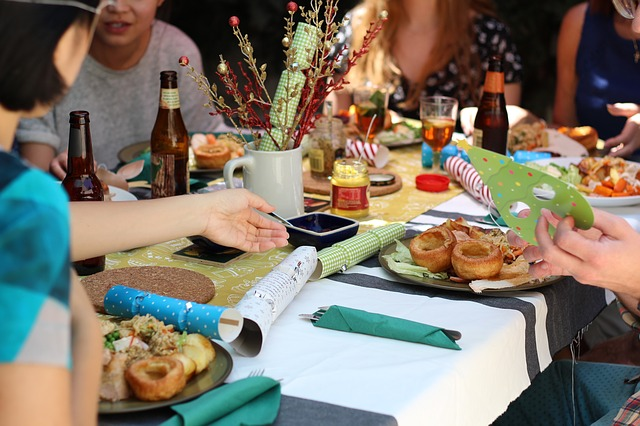
\includegraphics[width=450pt,]{images/1_01-friends.jpg}}}}{party}
\end{center}
\caption[{Digital made this gathering easier }]{Digital made this gathering easier \footnotemark{}}
\end{figure}
 
The resulting value is clear:
 \begin{itemize}

\item{} In an earlier era, our user might have stayed in, for fear of bouncing a check, or might have gone out and dined beyond her means.
 

\item{} The phone line at the restaurant might have been busy, so she might have risked showing up with no reservation.
 

\item{} Before texting and social media, she might not have been able to reach her friends as easily.
 

\item{} Without the traffic application she might have run into a huge midtown traffic jam and been half an hour late.
 
\end{itemize}
 
Clearly, information technology added value to her life and helped maximize her experiences of social enjoyment.
  
\subsubsection{Various forms of IT value}
\label{_various_forms_of_it_value}\hyperlabel{_various_forms_of_it_value}%
  
As we have seen, there are many ways in which digital systems deliver value. Some systems serve as the modern equivalent of file cabinets: massive and secure storage for financial transactions, insurance records, medical records, and the like. Other systems enable the transmission of information around the globe, whether as emails, web pages, voice calls, video on demand, or data to be displayed in a smart phone application ("app"). Some of these systems support engaged online communities and social interactions, with conversations, media sharing, and even massive online gaming ecosystems. Yet other systems enable penetrating analysis and insight, by examining the volumes of data contained in the first two kinds of systems for patterns and trends. Sophisticated statistical techniques and cutting edge approaches like neural network-{}based machine learning increase the insights our digital systems are capable of, at a seemingly exponential rate.
 
Digital technology generates value in both direct and indirect ways. People have long consumed (and paid for) communication services, such as telephone services. Broadcast entertainment was a different proposition, however. The "consumer" -{} the person with the radio or television -{} was not the "customer" -{} the person paying for the programming to go out over the airwaves. New business models sprung up to support the new media, through the sale of advertising air time. In other words, the value proposition was indirect, or at least took multiple parties to achieve: the listener, the broadcaster, and the advertiser. Finally, some of the best known uses of digital technology were and are very indirect -{} the above-{}mentioned banks and insurance agencies using the earliest computers to automate the work of thousands of typists and file clerks.
 
From these early business models have evolved and blossomed myriads of creative applications of digital technology, for the benefit of human beings in their ongoing pursuit of happiness and security. We see the applications mentioned at the outset: online banking, messaging, restaurant reservation, and traffic systems. Beyond that we see the use of digital technology in nearly every aspect of life. (And I say "nearly" only because I am a cautious person.)
 
Digital and information technology pervades all of the major industry verticals (manufacturing, agriculture, finance, retail, healthcare, transportation, services, and so on) and common industry functions (supply chain, human resources, corporate finance, and even IT itself).
 
Digital systems and technologies also are critical components of larger scale industrial, military, and aerospace systems. For better or worse, general purpose computers are increasingly found controlling safety-{}critical infrastructure, and serving as an intermediating layer between human actions and machine response. Robotic systems are based on software, and the Internet of Things ultimately will span billions of sensors and controllers in interconnected webs monitoring and adjusting all forms of complex operations across the planet.
   
\subsection{Defining Information Technology}
\label{_defining_information_technology}\hyperlabel{_defining_information_technology}%
  
\label{what-is-IT}\hyperlabel{what-is-IT}
 
\subsubsection{What is IT, anyways?}
\label{_what_is_it_anyways}\hyperlabel{_what_is_it_anyways}%
  
We've started this book in the previous section by providing an example of digital or IT value, without much discussion of how it is delivered. This is deliberate. But what is IT (Information Technology), anyways?
 \begin{itemize}

\item{} The computers? The networks?
 

\item{} The people who run them?
 

\item{} That organization under a Chief Information Officer that loves to say \textquotedblleft{}no\textquotedblright{} and is always slow and expensive?
 
\end{itemize}
 
None of these are how this book defines \textquotedblleft{}IT.\textquotedblright{} Although this is not a technical book on computer science or software engineering, the intent is that it reflects and is compatible with foundational principles.
 
\textquotedblleft{}Information technology\textquotedblright{} is ultimately based on the work of \href{https://en.wikipedia.org/wiki/Claude_Shannon}{Claude Shannon}, \href{https://en.wikipedia.org/wiki/Alan_Turing}{Alan Turing}, \href{https://en.wikipedia.org/wiki/Alonzo_Church}{Alonzo Church}, \href{https://en.wikipedia.org/wiki/John_von_Neumann}{John von Neumann}, and the other pioneers who defined the central problems of \href{https://en.wikipedia.org/wiki/Information_theory}{information theory}, \href{https://en.wikipedia.org/wiki/Digital_electronics}{digital logic},  \href{https://en.wikipedia.org/wiki/Computability}{computability}, and \href{https://en.wikipedia.org/wiki/Computer_architecture}{computer architecture}.
 
\label{IT-as-function}\hyperlabel{IT-as-function}
 
Additionally, as an organizational function, information technology also draws on organizational theory, systems theory, human factors and psychology, and more recent concepts such as design thinking, among many other areas.
 
Discussions of \textquotedblleft{}information technology\textquotedblright{} become contentious because some think of the traditional organization, while others think of the general problem area. IT has a long history as a corporate function, a single hierarchy under a powerful Chief Information Officer. This model has had its dysfunctions, including a longstanding reputation for being slow and expensive. Often, when one encounters the term \textquotedblleft{}IT,\textquotedblright{} the author using the term is referring to this organizational tradition.
 
\textbf{We are less interested in the future of IT as a distinct organizational structure. There are many different models, from fully centralized to fully embedded.} Organizational structure will be discussed in Chapter 7.
 
For this book, we define \textquotedblleft{}Information technology\textquotedblright{} in terms of its historic origins. We look to IT's common origins in automating the laborious and error prone processes of computation, through the application of digital logic technologies based on information transmission.
 
Regardless of organizational form or delivery methods, IT is defined by these origins. And there are notable common threads throughout this problem domain: the fragility and complexity of these systems, the need for layered abstractions in their management, and more.
 
It does not matter if the application developers ultimately report up through the CIO, the CMO, the CFO, or the COO. Their daily experience remains largely the same. The dynamics of their management remain the same. Executives who seek to take control of IT so they can \textquotedblleft{}remove that old bureaucracy\textquotedblright{} are well advised to be cautious; the bureaucracy emerged for a reason. More on this in subsequent chapters.
 
\label{digital-transformation}\hyperlabel{digital-transformation}
  
\subsubsection{IT and digital transformation}
\label{_it_and_digital_transformation}\hyperlabel{_it_and_digital_transformation}%
  \begin{quote}

IT doesn't matter.

\hspace*\fill--- Nicholas Carr
\end{quote}
 \begin{quote}

Software is eating the world.

\hspace*\fill--- Mark Andreessen
\end{quote}
 \begin{quote}

The digital realm is infusing the physical realm, like tea in hot water.

\hspace*\fill--- Jeff Sussna
\emph{Designing Delivery} \end{quote}
 
IT increasingly permeates business operations and social interactions. The breadth and depth of IT support for virtually all domains of society continues to expand. Lately, this is known as digital transformation.
 
The role of information technology seems critical to society and the economy, but there are various points of view. Nicholas Carr, in his controversial \emph{Harvard Business Review} article "IT Doesn't Matter," recognized that IT was becoming commoditized in an important sense \hyperlink{Carr2003}{[Carr2003]}. As Cloud providers started to offer utility-{}style computing, the choice of particular vendors of computers was no longer strategic. Looking to history, Carr argued that just as businesses no longer have \textquotedblleft{}Vice Presidents for Electricity,\textquotedblright{} so businesses no longer need Chief Information Officers or dedicated IT departments.
 \begin{DBKadmonition}{}{Note}
 
A "commodity" product is one that is offered from a variety of suppliers, with little or no difference between their offerings. Commodity products tend to compete on price, not on differences in features. Wheat is a commodity. Sports cars are not. "Commoditization" is the process by which products that used to compete by being different, increasingly compete on price.
 \end{DBKadmonition}
 
Carr has insight\hspace{0.167em}\textemdash{}\hspace{0.167em}there is no question IT is becoming pervasive\hspace{0.167em}\textemdash{}\hspace{0.167em}but he ultimately reflects a narrow view of what \textquotedblleft{}IT\textquotedblright{} is. If \textquotedblleft{}IT\textquotedblright{} were merely computation at the lowest level\hspace{0.167em}\textemdash{}\hspace{0.167em}just shuffling bits of information around, doing a little math\hspace{0.167em}\textemdash{}\hspace{0.167em}then perhaps it could be embedded throughout a business like electricity.
 
But IT has emergent aspects that are not comparable to electrical power. As it pervades all dimensions of business operations, it brings its concerns with it: complexity, fragility, and the skills required to cope with them.
 
One watt of electrical power is like any other watt of electrical power, and can usefully be seen as a commodity. We can use it to run toasters, hair dryers, or industrial paint mixers, and there is little concern (beyond supply and demand management) that the consumption of power by the paint mixer will affect the toaster.  It's also true that one cycle of computing, in a certain sense, is like any other cycle. But information technology systems interact with each other in surprising and unpredictable ways, orders of magnitude more complex than electrical power grids. (This is not to imply the modern electrical grid is a simple system!)
 
IT also radically transforms industries: from retail to transportation to manufacturing to genetics. Applied software-{}centric IT is unleashing remarkable economic disruption.
 
A lawyer may depend on a cell phone, and (in keeping with Carr) beyond its provision as a commodity service, needs little else to deliver the legal strategies a firm needs. A graphic designer may use computerized graphic tools, but these have become relatively standardized and commoditized in the past twenty years, and probably are not a source of competitive advantage in the quest for new marketing clients.
 
On the other hand, consider a text analytic algorithm that replaces thousands of paralegals, resulting in order-{}of-{}magnitude more accurate legal research in a fraction of cost and time. This \textbf{is} strategic and disruptive to the legal community. A superior supply chain algorithm, and the ability to improve it on an ongoing basis, may indeed elevate a logistics firm's performance above competitors. In cases like these\hspace{0.167em}\textemdash{}\hspace{0.167em}and they seem to be increasing\hspace{0.167em}\textemdash{}\hspace{0.167em}IT matters very much.
 
In the digitally transforming economy, traditional \textquotedblleft{}back office\textquotedblright{} IT organizations find themselves called on to envision, develop, and support market-{}facing applications of IT. And what starts with one market-{}facing use case can quickly expand into entire portfolios.  It is such cases that are of particular concern in this book.
 
Ultimately, it is possible that IT is the \textbf{most} strategic capability an organization can invest in. As the editor in chief of \emph{IEEE Software} notes \hyperlink{Spinellis2015}{[Spinellis2015]},
 \begin{quote}

other industries are also producing what's in effect software (executable knowledge) but not treating it as such . . . Although many industries have developed their own highly effective processes over the years, software engineering maintains an essential advantage. It has developed methods and tools that let even small teams manage extremely high complexity . . . This advantage is important because the complexity in non-{}software activities is also increasing inexorably . . . [T]he time has come to transform our world\ldots{} by giving back to science and technology the knowledge software engineering has produced.

\hspace*\fill--- Diomidis Spinellis
\emph{IEEE Software} \end{quote}
 
This ability to manage complexity, to turn tacit into explicit and formalize the previously unstructured, is an essential aspect of digital transformation.
  
\subsubsection{Defining "IT"}
\label{_defining_it}\hyperlabel{_defining_it}%
  
So, how do we define an IT problem, as opposed to other kinds of business problems? An IT problem is any problem where you are primarily constrained by your capability and understanding of IT.
 \begin{itemize}

\item{} If you need computer scientists or engineers who understand the fundamentals of information theory and computer science, you are doing IT.
 

\item{} If you need people who understand when your information-{}centric problems might need to be referred to such theorists and engineers, you are likely doing IT.
 

\item{} If you need people who are skilled in building upon those fundamentals, and operating technical platforms derived from them (such as programming languages, general purpose computers, and network routers), you are doing IT.
 
\end{itemize}
 
Regardless of whether IT is housed under a traditional CIO, an operations capability, a Chief Marketing Officer, or a \textquotedblleft{}line of business\textquotedblright{}, when it is critical to operations certain concerns inevitably follow:
 \begin{itemize}

\item{} Requirements (i.e. your intent for IT)
 

\item{} Sourcing and provisioning
 

\item{} IT-{}centric product design and construction
 

\item{} Configuration and change management
 

\item{} Support
 

\item{} Improvement
 
\end{itemize}
 
Executives who take control of information technology in hopes of making it more "agile" are often surprised to find that these concerns were not mere bureaucracy, but instead had well grounded origins in past failures. Ignoring these lessons is perilous.
 
And yet, the traditional, process-{}heavy IT organization does seem dysfunctional from a business point of view: a central theme of this book.
   
\subsection{IT services, systems, and applications}
\label{_it_services_systems_and_applications}\hyperlabel{_it_services_systems_and_applications}%
  
\subsubsection{Inside an IT service}
\label{_inside_an_it_service}\hyperlabel{_inside_an_it_service}%
  \begin{figure}[H]

\begin{center}
\imgexists{images/1.01-ITValue.png}{{\imgevalsize{images/1.01-ITValue.png}{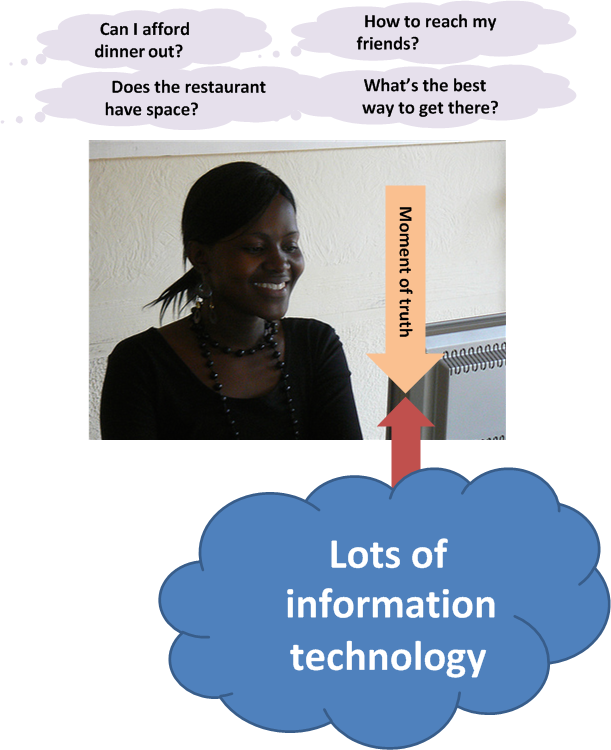
\includegraphics[width=400pt,]{images/1.01-ITValue.png}}}}{woman at computer}
\end{center}
\caption[{The basis of IT value }]{The basis of IT value \footnotemark{}}
\end{figure}
 
Let's examine our diner's value experience in more detail, without getting unnecessarily technical, and clarify some definitions along the way.  The first idea we need to cover is the "moment of truth." In terms of information technnology, this English-{}language clich� represents the user's experience of value.
 
In the example, our friend seeking a relaxing night out had several moments of truth:
 \begin{itemize}

\item{} Consulting her bank balance, and subsequent financial transactions also reflecting what was stated to her
 

\item{} Making a reservation and having it honored on arrival at the restaurant
 

\item{} Arriving on time to the restaurant, courtesy of the traffic application
 

\item{} And most importantly, having a relaxed and refreshing time with her friends.
 
\end{itemize}
 
Each of these individual value experiences was co-{}created by our friend's desire for value, and the response of a set of IT resources.
 \begin{DBKadmonition}{warning}{Important}
 
The "moment of truth" represents the user's experience of value, from a product, good, or service.
 \end{DBKadmonition}
 
In order to view her balance, our user is probably using an application downloaded from a "store" of applications made available to her device. On her device, this "app" is part of an intricate set of components performing functions such as:
 \begin{itemize}

\item{} accepting "input" (user intent) through a screen or voice input
 

\item{} processing that input through software and acting on her desire to see her bank balance
 

\item{} connecting to the phone network
 

\item{} securely connecting over the phone network to the Internet and then to the bank
 

\item{} identifying the user to the bank's systems
 

\item{} requesting the necessary information (in this case, an account balance)
 

\item{} receiving that information and converting it to a form that can be represented on a screeen
 

\item{} finally, displaying the information on the screen
 
\end{itemize}
 
The application, or "app," downloaded to the phone plays a primary role, but is enabled by:
 \begin{itemize}

\item{} the phone's operating system and associated services
 

\item{} the phone's hardware
 

\item{} the telecommunications infrastructure (cell phone towers, long distance fiber optic cables, switching offices, and much more)
 
\end{itemize}
 
Of course, without the banking systems on the other end, there is no bank balance to transmit. These systems are similar, but on a much larger scale than our friend's device:
 \begin{itemize}

\item{} Internet and middleware services to receive the request from the international network
 

\item{} Application services to validate the user's identity and route the request to the appropriate handling service
 

\item{} Data services to store the user's banking information (account identity and transactions) along with millions of other customers
 

\item{} Many additional services to detect fraud and security attacks, report on utilization, identify any errors in the systems, and much more.
 

\item{} Physical data centers full of computers and associated hardware including massive power and cooling infrastructure, and protected by security systems and personnel.
 
\end{itemize}
 
\begin{center}
 
\noindent\begin{minipage}[c]{\linewidth}
\begin{center}
\imgexists{images/1.01-ITStack.png}{{\imgevalsize{images/1.01-ITStack.png}{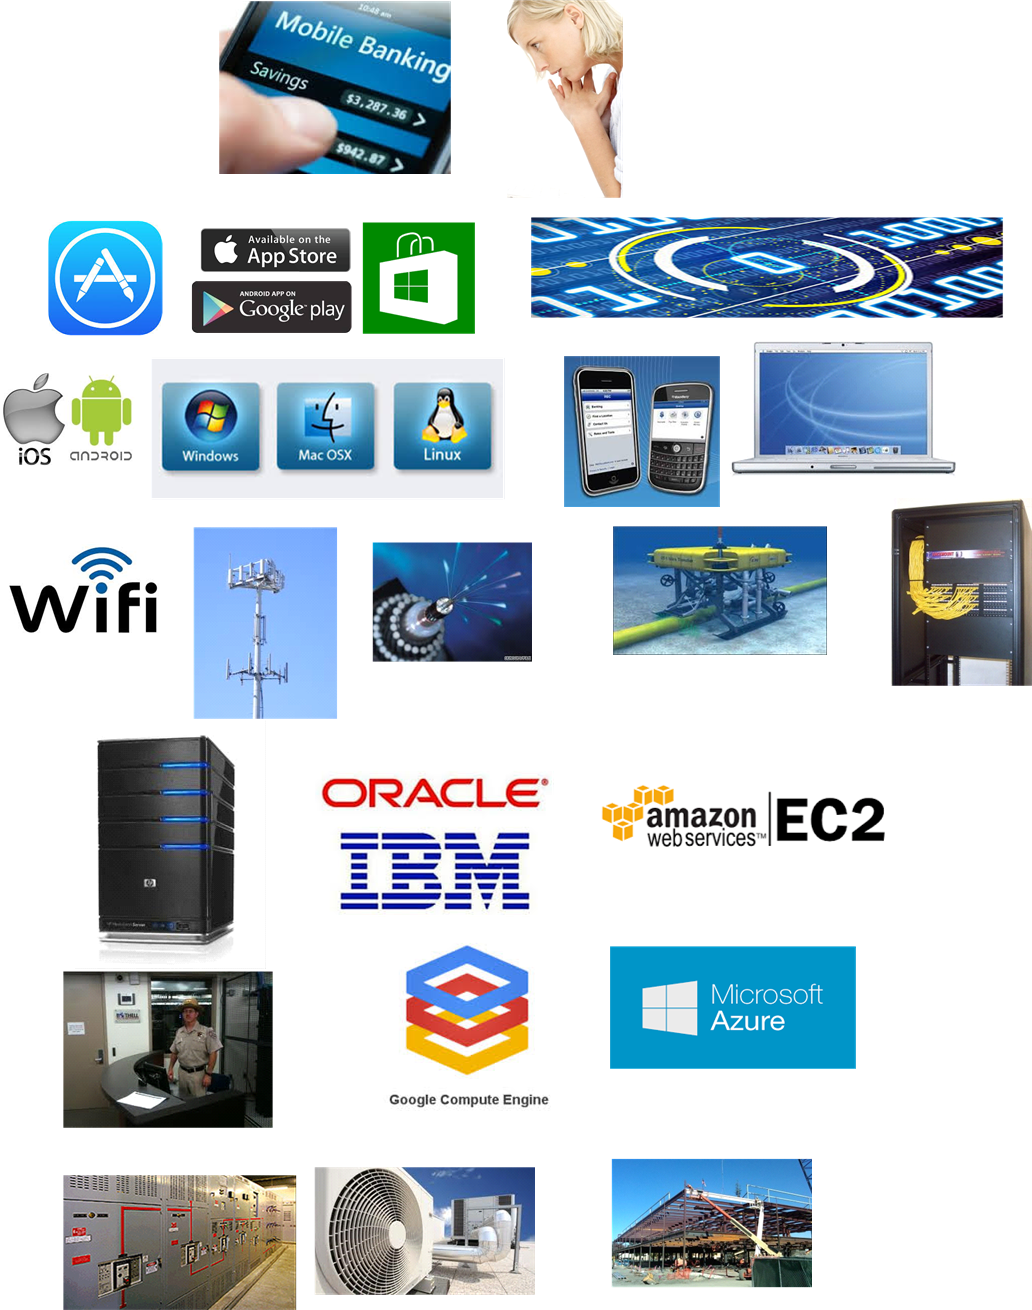
\includegraphics[width=\imgwidth,height=\imgheight,keepaspectratio=true]{images/1.01-ITStack.png}}}}{1.01 ITStack}\end{center}
\end{minipage}

 
\end{center}
 
Consider: what does all this mean to our user? Does she care about cell phone towers, or middleware, or triply-{}redundant industrial-{}strength Power Distribution Units? Usually, not in the least.
 
Therefore, as we study this world, we need to maintain awareness of her perspective. Our friend is seeking some value that IT uniquely can enable, but does not want to consider all the complexity that goes into it. She just wants to go out with friends. The moment of truth depends on the service; the service may contain great complexity, but part of its success lies in shielding the user from that complexity.
 
\begin{center}
 
\noindent\begin{minipage}[c]{\linewidth}
\begin{center}
\imgexists{images/1.01-ITStack2.png}{{\imgevalsize{images/1.01-ITStack2.png}{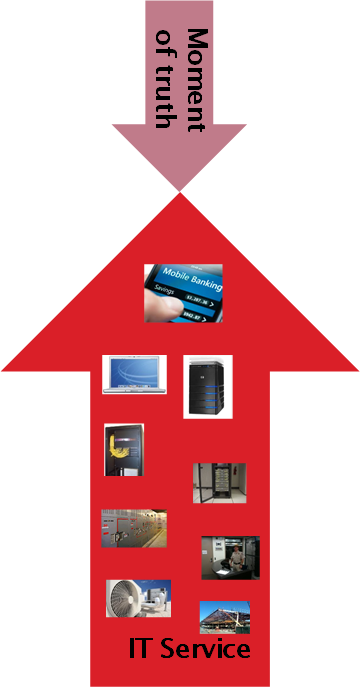
\includegraphics[width=\imgwidth,height=\imgheight,keepaspectratio=true]{images/1.01-ITStack2.png}}}}{1.01 ITStack2}\end{center}
\end{minipage}

 
\end{center}
 \begin{DBKadmonition}{warning}{Important}
 
Always remember the user's experience. Information technology has a well deserved reputation for being too complicated for end users\textemdash{}\hspace{0em}for example, trying to do something that should be simple, and finding oneself in a technical conversation about network settings.
 \end{DBKadmonition}
  
\subsubsection{What versus how}
\label{_what_versus_how}\hyperlabel{_what_versus_how}%
  
This fundamental tension between \textbf{what} a system is supposed to do, versus \textbf{how} it does it, pervades IT management and will likely define your career. "Don't trouble me with the details, just give me the results" is the overall theme, and we encounter this reaction to complexity in many aspects of life.
 
Terminology is important. We need to have a more precise way of describing the information technology, beyond just saying there is "lots" of it. A variety of terms are used in this text:
 \begin{itemize}

\item{} IT service
 

\item{} Application
 

\item{} IT system
 

\item{} IT infrastructure
 
\end{itemize}
 
We also see discussion of components, resources, subsystems, assets, and many more terms.
 \begin{DBKadmonition}{warning}{Warning}
 
There are many debates around these definitions. Sometimes these debates are helpful in clarifying the terminology you want to use on your team. But sometimes the debates don't add any value. Beware of anyone who claims there is a "best practice" here.
 \end{DBKadmonition}
 
In general, in this book, we will use the following definitions:
 \begin{itemize}

\item{} An IT service is defined primarily in terms of WHAT not HOW
 

\item{} Defining an IT system may include a discussion of both WHAT it does and HOW it does it
 

\item{} An "application" usually means some IT service or system for end users who are not primarily concerned with IT other than wanting to get something done with it (e.g. go out to dinner)
 

\item{} "Infrastructure" usually means some IT service or system that primarily supports OTHER IT services or systems (e.g. a network "service" is not usually useful to end users without additional application services.)
 
\end{itemize}
 
Finally, the concept of the "IT stack" is important. Notice how the different technology layers appear "stacked." Layered approaches to understanding IT are common; see Further Reading for useful references.
 

\begin{sidebar}
\textbf{Author's note: Service versus product}


For the purposes of this book, "IT services" are equivalent to "products." You may in other contexts hear phrases like "products \textbf{versus} services" which imply that they are distinct. Usually, when products are contrasted with services, people are equating products with goods: a jar of peanut butter is a "product," while a haircut is a service.

However, when I worked at AT\&T, the internal term for offerings like broadband networking access was not "service," but "product." Services, in this sense, \textbf{are} products.

In this book, we see products and services as roughly equivalent, but the two terms have some different connotations. Products usually imply an external market, where services can be either internal or external facing. While we certainly talk about "product marketing", the term "service marketing" is rarely seen. Furthermore,  some organizations such as Target have recently re-{}conceptualized internal services organizations as "product teams."
\end{sidebar}
    
\section{References}
\label{References}\hyperlabel{References}%
  \begin{DBKadmonition}{}{Note}
 
All web references were archived into the author's files on the indicated access date. Please contact the author if a link is broken.
 \end{DBKadmonition}
 \begin{itemize}

\item{} \label{Abbott2015}\hyperlabel{Abbott2015}[Abbott2015]: Abbott, Martin L.; Fisher, M.T., 2015. The Art of Scalability: Scalable Web Architecture, Processes, and Organizations for the Modern Enterprise (2nd Edition), Old Tappan, NJ, NJ: Pearson Education, Inc.
 

\item{} \label{Accounting2016}\hyperlabel{Accounting2016}[Accounting2016]: Accounting Coach. 2016. \textquotedblleft{}What Is Cost Accounting?\textquotedblright{} \href{http://www.accountingcoach.com/blog/what-is-cost-accounting}{http://www.accountingcoach.com/\-blog/\-what-{}is-{}cost-{}accounting} (May 7, 2016).
 

\item{} \label{Adzic2012}\hyperlabel{Adzic2012}[Adzic2012]: Adzic, Gojko. 2012. Impact Mapping: Making a Big Impact with Software Products and Projects. Gojko Adzic.
 

\item{} \label{Akera2007}\hyperlabel{Akera2007}[Akera2007]: Akera, A., "Edmund Berkeley and the Origins of the ACM." Communications of the ACM, 2007. 50(5): p. 31-{}35.
 

\item{} \label{Alliance2001}\hyperlabel{Alliance2001}[Alliance2001]: Agile Alliance. (2001), "Agile Manifesto and Principles", \href{http://agilemanifesto.org/principles.html}{http://agilemanifesto.org/\-principles.html}
 

\item{} \label{Alliance2015}\hyperlabel{Alliance2015}[Alliance2015]: Agile Alliance. 2015. \textquotedblleft{}Team Definition.\textquotedblright{} Glossary. \href{https://www.agilealliance.org/glossary/team/}{https://www.agilealliance.org/\-glossary/\-team/\-}. Accessed 2016-{}09-{}21.
 

\item{} \label{Alliance2015a}\hyperlabel{Alliance2015a}[Alliance2015a]: Agile Alliance. 2016. \textquotedblleft{}Definition of Done.\textquotedblright{} Glossary. \href{https://www.agilealliance.org/glossary/definition-of-done/#sthash.6rSCZMyU.dpuf}{https://www.agilealliance.org/\-glossary/\-definition-{}of-{}done/\-\#sthash.6rSCZMyU.dpuf}.
 

\item{} \label{Alliance2016}\hyperlabel{Alliance2016}[Alliance2016]: Agile Alliance, 2016. Definition of Done. Glossary. Available at: \href{https://www.agilealliance.org/glossary/definition-of-done/#sthash.6rSCZMyU.dpuf}{https://www.agilealliance.org/\-glossary/\-definition-{}of-{}done/\-\#sthash.6rSCZMyU.dpuf} [Accessed November 16, 2016].
 

\item{} \label{Allspaw2009}\hyperlabel{Allspaw2009}[Allspaw2009]: Allspaw, J. \& Hammond, P. (2009), "10 deploys per day: Dev \& ops cooperation at Flickr",  O'Reilly Publications, \href{http://www.slideshare.net/jallspaw/10-deploys-per-day-dev-and-ops-cooperation-at-flickr}{http://www.slideshare.net/\-jallspaw/\-10-{}deploys-{}per-{}day-{}dev-{}and-{}ops-{}cooperation-{}at-{}flickr}
 

\item{} \label{Ambler2005}\hyperlabel{Ambler2005}[Ambler2005]: Ambler, S. (2005) "Agile Outsourcing." \emph{Dr. Dobb's Journal}.  Retrieved from \href{http://www.drdobbs.com/architecture-and-design/agile-outsourcing/184415344}{http://www.drdobbs.com/\-architecture-{}and-{}design/\-agile-{}outsourcing/\-184415344}. Date Accessed:  3/21/2016.
 

\item{} \label{Ambler2006}\hyperlabel{Ambler2006}[Ambler2006]: Ambler, Scott W, and Pramod J Sadalage. 2006. Refactoring Databases : Evolutionary Database Design. Book. Harlow, U.K.: Addison-{}Wesley. Table of contents \href{http://www.loc.gov/catdir/toc/ecip063/2005031959.html}{http://www.loc.gov/\-catdir/\-toc/\-ecip063/\-2005031959.html}.
 

\item{} \label{Ambler2012}\hyperlabel{Ambler2012}[Ambler2012]: Ambler, Scott W, and Mark Lines. 2012. Disciplined Agile Delivery: A Practitioner's Guide to Agile Software Delivery in the Enterprise. IBM Press.
 

\item{} \label{Anderson2010}\hyperlabel{Anderson2010}[Anderson2010]: Anderson, D. J. (2010), \emph{Kanban: Successful Evolutionary Change for your Technology Business}, Blue Hole Press, Sequim, WA
 

\item{} \label{Arbogast2012}\hyperlabel{Arbogast2012}[Arbogast2012]: Arbogast, T. L., Craig; Vodde, Bas (2012) "Agile Contracts Primer."  Retrieved from \href{http://www.agilecontracts.com/agile_contracts_primer.pdf}{http://www.agilecontracts.com/\-agile\_contracts\_primer.pdf}. Date Accessed:  March 21, 2016.
 

\item{} \label{Arnold2013}\hyperlabel{Arnold2013}[Arnold2013]: Arnold, J., 2013. Tilt the playing field: discover, nurture, and speed up the delivery of value. Available at: \href{https://liber.io/v/liberioEpub_53aa4d19e3a7e}{https://liber.io/\-v/\-liberioEpub\_53aa4d19e3a7e}.
 

\item{} \label{Ashmore2014}\hyperlabel{Ashmore2014}[Ashmore2014]: Ashmore, S. and K. Runyan, 2014, \emph{Introduction to agile methods}. xix, 307 pages.
 

\item{} \label{Bacik2011}\hyperlabel{Bacik2011}[Bacik2011]: Bacik, S. (2011). Compliance, audit, risk, security \textendash{} what's the difference and why do we need it? Retrieved July 6, 2016, from \href{http://www.enernex.com/wp-content/uploads/2011/11/Risk-Compliance-Audit-webinar-11.2011.pdf}{http://www.enernex.com/\-wp-{}content/\-uploads/\-2011/\-11/\-Risk-{}Compliance-{}Audit-{}webinar-{}11.2011.pdf}
 

\item{} \label{BAGuild2016}\hyperlabel{BAGuild2016}[BAGuild2016]: Business Architecture Guild. 2016. A Guide to the Business Architecture Body of Knowledge (BIZBOK Guide). Business Architecture Guild.
 

\item{} \label{Bank2016}\hyperlabel{Bank2016}[Bank2016]: Bank, C., \& Cao, J. (n.d.). The Guide to Usability Testing. uxpin.com. Retrieved from \href{https://www.uxpin.com/studio/ebooks/guide-to-usability-testing/}{https://www.uxpin.com/\-studio/\-ebooks/\-guide-{}to-{}usability-{}testing/\-} (free ebook, accessed 2016-{}09-{}22)
 

\item{} \label{Beck2000}\hyperlabel{Beck2000}[Beck2000]: Beck, K., 2000 \emph{extreme programming eXplained : embrace change}, Reading, MA: Addison-{}Wesley. xxi, 190 p.
 

\item{} \label{Bell2010}\hyperlabel{Bell2010}[Bell2010]: Bell, S. C. \& Orzen, M. A. (2010), \emph{Lean IT}, CRC Press, Boca Raton, Florida
 

\item{} \label{Bell2013}\hyperlabel{Bell2013}[Bell2013]: Bell, Steve et al. 2013. \emph{Run Grow Transform: Integrating Business and Lean IT}. Boca Raton, FL: CRC Press.
 

\item{} \label{Bente2012}\hyperlabel{Bente2012}[Bente2012]: Bente, Stefan, Uwe Bombosch, and Shailendra Langade. 2012. Collaborative Enterprise Architecture: Enriching EA with Lean, Agile, and Enterprise 2.0 Practices. Waltham, MA: Morgan Kaufman -{} Elsevier.
 

\item{} \label{Bernard2012}\hyperlabel{Bernard2012}[Bernard2012]: Bernard, Scott. 2012. An Introduction to Enterprise Architecture. AuthorHouse.
 

\item{} \label{Betz2011}\hyperlabel{Betz2011}[Betz2011]: Betz, C. (2011), "Release management integration pattern -{} seeking devops comments", \href{http://www.lean4it.com/2011/01/release-management-integration-pattern-seeking-devops-comments.html}{http://www.lean4it.com/\-2011/\-01/\-release-{}management-{}integration-{}pattern-{}seeking-{}devops-{}comments.html}
 

\item{} \label{Betz2011a}\hyperlabel{Betz2011a}[Betz2011a]: Betz, C. T. (2011), \emph{Architecture and Patterns for IT: Service and Portfolio Management and Governance (Making Shoes for the Cobbler's Children), 2nd Edition}, Elsevier/Morgan Kaufman, Amsterdam
 

\item{} \label{Betz2011b}\hyperlabel{Betz2011b}[Betz2011b]:Betz, C. (2011). "ITIL�, COBIT�, and CMMI�: Ongoing Confusion of Process and Function."" BPTrends. Retrieved from \href{http://www.bptrends.com/publicationfiles/10-04-2011-ART-Ongoing}{http://www.bptrends.com/\-publicationfiles/\-10-{}04-{}2011-{}ART-{}Ongoing} Confusion of Process and Function-{}Betz-{}Final.pdf
 

\item{} \label{Betz2015}\hyperlabel{Betz2015}[Betz2015]: Betz, C.T. (2015), "Calavera project", Github, \href{https://github.com/CharlesTBetz/Calavera}{https://github.com/\-CharlesTBetz/\-Calavera}
 

\item{} \label{Beyer2016}\hyperlabel{Beyer2016}[Beyer2016]: Beyer, B., Jones, C., Petoff, J., \& Murphy, N. R. (2016). Site Reliability Engineering: How Google Runs Production Systems. Sebastopol, CA, CA: O'Reilly Media, Inc.
 

\item{} \label{Bias2012}\hyperlabel{Bias2012}[Bias2012]: Bias, R. (2012, February 14). Architectures for open and scalable clouds. Retrieved November 10, 2016, from \href{http://www.slideshare.net/randybias/architectures-for-open-and-scalable-clouds}{http://www.slideshare.net/\-randybias/\-architectures-{}for-{}open-{}and-{}scalable-{}clouds}
 

\item{} \label{Binder1997}\hyperlabel{Binder1997}[Binder1997]: Binder, R.V. 1997. \textquotedblleft{}Can a Manufacturing Quality Model Work for Software?\textquotedblright{} IEEE Software 14 (5). IEEE: 101\textendash{}2, 105. doi:10.1109/52.605937.
 

\item{} \label{Blank2013}\hyperlabel{Blank2013}[Blank2013]: Blank, Steve. 2013. The Four Steps to the Epiphany: Successful Strategies for Products That Win. 2nd ed. Steve Blank, publisher.
 

\item{} \label{Bloomberg2014}\hyperlabel{Bloomberg2014}[Bloomberg2014]: Bloomberg, Jason. 2014. \textquotedblleft{}Agile Enterprise Architecture Finally Crosses the Chasm.\textquotedblright{} Forbes. July. \href{http://www.forbes.com/sites/jasonbloomberg/2014/07/23/agile-enterprise-architecture-finally-crosses-the-chasm/print/}{http://www.forbes.com/\-sites/\-jasonbloomberg/\-2014/\-07/\-23/\-agile-{}enterprise-{}architecture-{}finally-{}crosses-{}the-{}chasm/\-print/\-}. Accessed 2015-{}11-{}12.
 

\item{} \label{BPTrends2013}\hyperlabel{BPTrends2013}[BPTrends2013]: BPTrends. 2013. \textquotedblleft{}Scope Diagram (or Input-{}Guides-{}Outputs-{}Enablers \textendash{} IGOE Diagram).\textquotedblright{} BPTrends. \href{http://www.bptrends.com/resources/glossary/scope-diagram-or-input-guides-outputs-enablers-igoe-diagram/}{http://www.bptrends.com/\-resources/\-glossary/\-scope-{}diagram-{}or-{}input-{}guides-{}outputs-{}enablers-{}igoe-{}diagram/\-}.
 

\item{} \label{Brooks1995}\hyperlabel{Brooks1995}[Brooks1995]: Brooks, Frederick P. 1995. \emph{The Mythical Man-{}Month: Essays on Software Engineering.} 25th Anniversary edition. Reading, Mass.: Addison-{}Wesley Pub. Co.
 

\item{} \label{Bossavit2015}\hyperlabel{Bossavit2015}[Bossavit2015]:	Bossavit, L., 2015. \emph{The Leprechauns of Software Engineering: How folklore turns into fact and what to do about it} 2015. Available from: \href{https://leanpub.com/leprechauns}{https://leanpub.com/\-leprechauns}.
 

\item{} \label{Bouwman}\hyperlabel{Bouwman}[Bouwman]: Bouwman, J.-{}J. \& Heistek, M. (), "ITIL and DevOps at war in the enterprise,"" \href{https://www.youtube.com/watch?v=_dDsdbkSgOc}{https://www.youtube.com/\-watch?v=\_dDsdbkSgOc}, 'DevOpsDays'.
 

\item{} \label{Brooks1975}\hyperlabel{Brooks1975}[Brooks1975]: Brooks, F. P. (1975). \emph{The mythical man-{}month: essays on software engineering.} Reading, Mass., Addison-{}Wesley Pub. Co.
 

\item{} \label{Brustein2013}\hyperlabel{Brustein2013}[Brustein2013]: Brustein, Joshua. 2013. \textquotedblleft{}Microsoft Kills Its Hated Stack Rankings. Does Anyone Do Employee Reviews Right?\textquotedblright{} Bloomberg Business Week. \href{http://www.bloomberg.com/news/articles/2013-11-13/microsoft-kills-its-hated-stack-rankings-dot-does-anyone-do-employee-reviews-right}{http://www.bloomberg.com/\-news/\-articles/\-2013-{}11-{}13/\-microsoft-{}kills-{}its-{}hated-{}stack-{}rankings-{}dot-{}does-{}anyone-{}do-{}employee-{}reviews-{}right} (March 5, 2016).
 

\item{} \label{Buchholz1962}\hyperlabel{Buchholz1962}[Buchholz1962]: Buchholz, Werner. 1962. Planning a Computer System: Project Stretch. New York: McGraw-{}Hill Book Company, Inc.
 

\item{} \label{Buckingham2015}\hyperlabel{Buckingham2015}[Buckingham2015]: Buckingham, Marcus, and Ashley Goodall. 2015. \textquotedblleft{}Reinventing Performance Management.\textquotedblright{} Harvard Business Review 93(4): 40\textendash{}50. \href{https://hbr.org/2015/04/reinventing-performance-management}{https://hbr.org/\-2015/\-04/\-reinventing-{}performance-{}management}.
 

\item{} \label{Burlton2001}\hyperlabel{Burlton2001}[Burlton2001]: Burlton, Roger. 2001. \emph{Business Process Management: Profiting from Process}. Indianapolis, Indiana: SAMS.
 

\item{} \label{Burgess2015}\hyperlabel{Burgess2015}[Burgess2015]: Burgess, Mark. 2015. \emph{Thinking in Promises}. Sebastopol, CA: O'Reilly Media.
 

\item{} \label{Burgess2016}\hyperlabel{Burgess2016}[Burgess2016]: Burgess, Mark. Undated. \textquotedblleft{}When and Where Order Matters.\textquotedblright{} Homepage Mark Burgess. Accessed November 12 2016. \href{http://markburgess.org/blog_order.html}{http://markburgess.org/\-blog\_order.html}.
 

\item{} \label{Burrows2006}\hyperlabel{Burrows2006}[Burrows2006]: Burrows, M. G. I. (2006). "The Chubby lock service for loosely-{}coupled distributed systems." 7th symposium on Operating systems design and implementation (OSDI '06), USENIX Association Berkeley, CA, USA
 

\item{} \label{Burrows2014}\hyperlabel{Burrows2014}[Burrows2014]: Burrows, Mike. (2014) \emph{Kanban from the Inside: Understand the Kanban Method, connect it to what you already know, introduce it with impact}. Sequim, WA, Blue Hole Press.
 

\item{} \label{Buschmann1996}\hyperlabel{Buschmann1996}[Buschmann1996]: Buschmann, F. (1996), \emph{Pattern-{}oriented software architecture : a system of patterns}, Wiley, Chichester ; New York
 

\item{} \label{Butler2013}\hyperlabel{Butler2013}[Butler2013]: Butler, Brandon. 2013. \textquotedblleft{}Free Cloud Storage Service MegaCloud Goes Dark.\textquotedblright{} Network World. doi:http://www.networkworld.com/article/2171450/cloud-{}computing/free-{}cloud-{}storage-{}service-{}megacloud-{}goes-{}dark.html. Accessed 2016-{}07-{}01.
 

\item{} \label{Butler2014}\hyperlabel{Butler2014}[Butler2014]: Butler, Brandon. 2014. \textquotedblleft{}Cloud's Worst-{}Case Scenario: What to Do If Your Provider Goes Belly up.\textquotedblright{} Network World. \href{http://www.networkworld.com/article/2173255/cloud-computing/cloud-s-worst-case-scenario-what-to-do-if-your-provider-goes-belly-up.html.Accessed}{http://www.networkworld.com/\-article/\-2173255/\-cloud-{}computing/\-cloud-{}s-{}worst-{}case-{}scenario-{}what-{}to-{}do-{}if-{}your-{}provider-{}goes-{}belly-{}up.html.Accessed} 2016-{}07-{}01.
 

\item{} \label{Cadbury1992}\hyperlabel{Cadbury1992}[Cadbury1992]: Committee on the Financial Aspects of Corporate Governance. 1992. \textquotedblleft{}Report of the Committee on the Financial Aspects of Corporate Governance (aka Cadbury Report).\textquotedblright{} London, Gee \& Co. Ltd.
 

\item{} \label{Cagan2008}\hyperlabel{Cagan2008}[Cagan2008]: Cagan, Marty. 2008. Inspired: How to Create Products Customers Love. SVPG Press. \href{http://www.amazon.com/Inspired-Create-Products-Customers-Love/dp/0981690408}{http://www.amazon.com/\-Inspired-{}Create-{}Products-{}Customers-{}Love/\-dp/\-0981690408}.
 

\item{} \label{Card1999}\hyperlabel{Card1999}[Card1999]: Card, S. K., Mackinlay, J. D., \& Shneiderman, B. (1999). Readings in Information Visualization: Using Vision to Think. San Diego: Academic Press.
 

\item{} \label{Carr2003}\hyperlabel{Carr2003}[Carr2003]: Carr, N. (2003). IT Doesn't Matter. Harvard Business Review, 5\textendash{}12.
 

\item{} \label{Carroll2013}\hyperlabel{Carroll2013}[Carroll2013]: Carroll, I. (2013), "Various", \href{http://itopskanban.wordpress.com/before/}{http://itopskanban.wordpress.com/\-before/\-}
 

\item{} \label{Castaldo2016}\hyperlabel{Castaldo2016}[Castaldo2016]: Castaldo, Joe. 2016. \textquotedblleft{}The Last Days of Target: The Untold Tale of Target Canada's Difficult Birth, Tough Life and Brutal Death.\textquotedblright{} Canadian Business. \href{http://www.canadianbusiness.com/the-last-days-of-target-canada/}{http://www.canadianbusiness.com/\-the-{}last-{}days-{}of-{}target-{}canada/\-}. Accessed 2016-{}08-{}30.
 

\item{} \label{Chacon2009}\hyperlabel{Chacon2009}[Chacon2009]: Chacon, S. \& Straub, B. (2009). Pro Git. Berkeley, CA. New York, Apress.
 

\item{} \label{Cherubini2007}\hyperlabel{Cherubini2007}[Cherubini2007]: Cherubini, M., Venolia, G., Deline, R., \& Ko, A. J. (2007). Let ' s Go to the Whiteboard: How and Why Software Developers Use Drawings. CHI 2007 Proceedings, 557\textendash{}566. \href{http://doi.org/10.1145/1240624.1240714}{http://doi.org/\-10.1145/\-1240624.1240714}. \href{https://www.microsoft.com/en-us/research/wp-content/uploads/2016/02/p557-cherubini.pdf}{https://www.microsoft.com/\-en-{}us/\-research/\-wp-{}content/\-uploads/\-2016/\-02/\-p557-{}cherubini.pdf}, accessed 2016-{}10-{}17.
 

\item{} \label{Chisholm2001}\hyperlabel{Chisholm2001}[Chisholm2001]: Chisholm, M. (2001). Managing Reference Data in Enterprise Databases: Binding Corporate Data to the Wider World. San Diego: Academic Press.
 

\item{} \label{Christensen2006}\hyperlabel{Christensen2006}[Christensen2006]: Christensen, Clayton, Scott Cook, and Taddy Hall. 2006. \textquotedblleft{}What Customers Want from Your Products.\textquotedblright{} Working Knowledge (Harvard Business School). \href{http://hbswk.hbs.edu/item/what-customers-want-from-your-products}{http://hbswk.hbs.edu/\-item/\-what-{}customers-{}want-{}from-{}your-{}products}. Accessed 2016-{}09-{}18.
 

\item{} \label{Christensen2015}\hyperlabel{Christensen2015}[Christensen2015]: Clayton Christensen Institute. 2015. \textquotedblleft{}Jobs to Be Done.\textquotedblright{} Http://www.christenseninstitute.org/. \href{http://www.christenseninstitute.org/key-concepts/jobs-to-be-done/}{http://www.christenseninstitute.org/\-key-{}concepts/\-jobs-{}to-{}be-{}done/\-}. Accessed 2016-{}09-{}18.
 

\item{} \label{Clark2006}\hyperlabel{Clark2006}[Clark2006]: Clark, Nicola. 2006. \textquotedblleft{}The Airbus Saga: Crossed Wires and a Multibillion-{}Euro Delay.\textquotedblright{} New York Times, December 11. \href{http://www.nytimes.com/2006/12/11/business/worldbusiness/11iht-airbus.3860198.html}{http://www.nytimes.com/\-2006/\-12/\-11/\-business/\-worldbusiness/\-11iht-{}airbus.3860198.html}. Accessed 2016-{}10-{}11.
 

\item{} \label{Coase1937}\hyperlabel{Coase1937}[Coase1937]: Coase, R. (1937). The nature of the firm. \emph{Economica}, 4, 386\textendash{}405.
 

\item{} \label{Cobb2015}\hyperlabel{Cobb2015}[Cobb2015]: Cobb, C.G., (2015), \emph{The Project MANAGER'S GUIDE TO MASTERING AGILE: Principles and Practices for an Adaptive Approach}, Hoboken, New Jersey: John Wiley \& Sons.
 

\item{} \label{Cockburn2007}\hyperlabel{Cockburn2007}[Cockburn2007]: Cockburn, Alistair. 2007. Agile Software Development: The Cooperative Game. 2nd ed. Boston, MA: Pearson Education, Inc.
 

\item{} \label{Cohn2010}\hyperlabel{Cohn2010}[Cohn2010]: Cohn, M., \emph{Succeeding with Agile: Software Development Using Scrum}, Addison-{}Wesley: Upper Saddle River, New Jersey.
 

\item{} \label{Comella2016}\hyperlabel{Comella2016}[Comella2016]: Comella-{}Dorda, Santiago, Lohiya, Swati, and Gerard Speksnijder. 2016. \textquotedblleft{}An Operating Model for Company-{}Wide Agile Development.\textquotedblright{} McKinsey \& Company. \href{http://www.mckinsey.com/Business-Functions/Business-Technology/Our-Insights/An-operating-model-for-company-wide-agile-development}{http://www.mckinsey.com/\-Business-{}Functions/\-Business-{}Technology/\-Our-{}Insights/\-An-{}operating-{}model-{}for-{}company-{}wide-{}agile-{}development}.
 

\item{} \label{Conway1968}\hyperlabel{Conway1968}[Conway1968]: Conway, D.M.E., 1968. How Do Committees Invent? Available at: \href{http://www.melconway.com/research/committees.html}{http://www.melconway.com/\-research/\-committees.html} [Accessed November 25, 2016].
 

\item{} \label{Cooper2009}\hyperlabel{Cooper2009}[Cooper2009]: Cooper, A., Reimann, R., \& Cronin, D. (2009). About Face 3: The Essentials of Interaction Design. online. Retrieved from \href{http://www.amazon.com/About-Face-Essentials-Interaction-Design-ebook/dp/B008NC0XR2/}{http://www.amazon.com/\-About-{}Face-{}Essentials-{}Interaction-{}Design-{}ebook/\-dp/\-B008NC0XR2/\-}
 

\item{} \label{COSO2013}\hyperlabel{COSO2013}[COSO2013]: Committee of Sponsoring Organizations of the Treadway Commission. 2013. \textquotedblleft{}Internal Control \textemdash{} Integrated Framework (Executive Summary).\textquotedblright{} \href{http://www.coso.org/documents/990025P_Executive_Summary_final_may20_e.pdf}{http://www.coso.org/\-documents/\-990025P\_Executive\_Summary\_final\_may20\_e.pdf}.
 

\item{} \label{Csikszentmihalyi1990}\hyperlabel{Csikszentmihalyi1990}[Csikszentmihalyi1990]: Csikszentmihalyi, M. (1990). Flow : the psychology of optimal experience. New York, Harper \& Row.
 

\item{} \label{Cunningham1992}\hyperlabel{Cunningham1992}[Cunningham1992]: Cunningham, Ward. 1992. \textquotedblleft{}Experience Report: The WyCash Portfolio Management System.\textquotedblright{} OOPSLA '92. \href{http://c2.com/doc/oopsla92.html}{http://c2.com/\-doc/\-oopsla92.html}. Accessed 2016-{}10-{}6.
 

\item{} \label{DAMA2009}\hyperlabel{DAMA2009}[DAMA2009]: Data Management Association, The. 2009. The DAMA Guide to The Data Management Body of Knowledge (DAMA-{}DMBOK Guide). Bradley Beach, NJ: Technics Publications, LLC.
 

\item{} \label{Davenport2007}\hyperlabel{Davenport2007}[Davenport2007]: Davenport, Thomas H, and Jeanne G Harris. 2007. Competing on Analytics : The New Science of Winning. Boston, Mass.: Harvard Business School ; London : McGraw-{}Hill [distributor]. Table of contents only \href{http://www.loc.gov/catdir/toc/ecip073/2006035422.html}{http://www.loc.gov/\-catdir/\-toc/\-ecip073/\-2006035422.html}.
 

\item{} \label{Dekker2006}\hyperlabel{Dekker2006}[Dekker2006]: Dekker, S. (2006). The Field Guide to Understanding Human Error. book, Burlington, VT: Ashgate Publishing Limited.
 

\item{} \label{delaMaza2016}\hyperlabel{delaMaza2016}[delaMaza2016]: de la Maza, Michael, and David Benz. 2016. Why Agile Works: The Values Behind the Results. C4Media -{} InfoQ.com. \href{http://www.infoq.com/resource/minibooks/why-agile-works}{http://www.infoq.com/\-resource/\-minibooks/\-why-{}agile-{}works}. Accessed 2016-{}10-{}11.
 

\item{} \label{DeLuccia2008}\hyperlabel{DeLuccia2008}[DeLuccia2008]: DeLuccia, James. 2008. \emph{IT COMPLIANCE AND CONTROLS: Best Practices for Implementation}. Hoboken, N.J.: John Wiley \& Sons, Inc.
 

\item{} \label{DeLuccia2015}\hyperlabel{DeLuccia2015}[DeLuccia2015]: DeLuccia, James, Jeff Gallimore, Gene Kim, and Byron Miller. 2015. \textquotedblleft{}DevOps Audit Defense Toolkit.\textquotedblright{} \href{http://itrevolution.com/devops-and-auditors-the-devops-audit-defense-toolkit/}{http://itrevolution.com/\-devops-{}and-{}auditors-{}the-{}devops-{}audit-{}defense-{}toolkit/\-}.
 

\item{} \label{DeNicola216}\hyperlabel{DeNicola216}[DeNicola216]: De Nicola, Antonio, and Michelle Missikoff. 2016. \textquotedblleft{}A Lightweight Methodology for Rapid Ontology Engineering.\textquotedblright{} Communications of the ACM2 59 (3): 79\textendash{}86.
 

\item{} \label{DHS2006}\hyperlabel{DHS2006}[DHS2006]: Department of Homeland Security. 2006. \textquotedblleft{}Report No. 2006-{}03, The Use of Commercial Data.\textquotedblright{} DHS Data Privacy and Integrity Advisory Committee.
 

\item{} \label{Ditri1971}\hyperlabel{Ditri1971}[Ditri1971]: Ditri, A.E., Shaw, J.C. \& Atkins, W., 1971. Managing the EDP function, N.Y.: McGraw-{}Hill.
 

\item{} \label{Drucker1963}\hyperlabel{Drucker1963}[Drucker1963]: Drucker, Peter F. 1963. \textquotedblleft{}Managing for Business Effectiveness.\textquotedblright{} Magazine Article. Harvard Business Review.
 

\item{} \label{Drucker1993}\hyperlabel{Drucker1993}[Drucker1993]: Drucker, Peter F. 1993. \emph{Post-{}Capitalist Society}. 1st ed. New York, NY: HarperBusiness.
 

\item{} \label{duPreez2015}\hyperlabel{duPreez2015}[duPreez2015]: du Preez, Derek. 2015. \textquotedblleft{}A CIO's Worst Nightmare: When Your Cloud Provider Goes Bankrupt.\textquotedblright{} Diginomica. \href{http://diginomica.com/2015/01/06/cios-worst-nightmare-cloud-provider-goes-bankrupt/}{http://diginomica.com/\-2015/\-01/\-06/\-cios-{}worst-{}nightmare-{}cloud-{}provider-{}goes-{}bankrupt/\-}. Accessed 2016-{}07-{}04.
 

\item{} \label{Duvall2007}\hyperlabel{Duvall2007}[Duvall2007]: Duvall, P. M.; Matyas, S. \& Glover, A. (2007), \emph{Continuous integration : improving software quality and reducing risk}, Addison-{}Wesley, Upper Saddle River, NJ
 

\item{} \label{Edwards2012}\hyperlabel{Edwards2012}[Edwards2012]: Edwards, D. (2012), "Integrating DevOps tools into a Service Delivery Platform", \href{http://dev2ops.org/2012/07/integrating-devops-tools-into-a-service-delivery-platform-video/}{http://dev2ops.org/\-2012/\-07/\-integrating-{}devops-{}tools-{}into-{}a-{}service-{}delivery-{}platform-{}video/\-}
 

\item{} \label{Eisenhardt1989}\hyperlabel{Eisenhardt1989}[Eisenhardt1989]: Eisenhardt, Kathleen M. 1989. \textquotedblleft{}Agency Theory: An Assessment and Review.\textquotedblright{} \emph{Academy of Management Review} 14 (1): 57\textendash{}74. \href{http://www.jstor.org/stable/258191}{http://www.jstor.org/\-stable/\-258191}.
 

\item{} \label{England2013}\hyperlabel{England2013}[England2013]: England, Rob. 2013. \emph{Plus! The Standard+Case Approach: See Service Response in a New Light}. Mana, New Zealand: Two Hills Ltd.
 

\item{} \label{Evans2004}\hyperlabel{Evans2004}[Evans2004]: Evans, Eric. 2004. Domain-{}Driven Design : Tackling Complexity in the Heart of Software. Book. Boston ; London: Addison-{}Wesley.
 

\item{} \label{Fisher2016}\hyperlabel{Fisher2016}[Fisher2016]: Fisher, T. (2016). Designing Our Way to a Better World. Minneapolis, MN: University of Minnesota Press.
 

\item{} \label{Flahiff2016}\hyperlabel{Flahiff2016}[Flahiff2016]: Flahiff, J. (2016). "How organizational agility will save and destroy your company." from \href{http://searchcio.techtarget.com/tip/How-organizational-agility-will-save-and-destroy-your-company}{http://searchcio.techtarget.com/\-tip/\-How-{}organizational-{}agility-{}will-{}save-{}and-{}destroy-{}your-{}company}. Accessed March 19, 2016.
 

\item{} \label{Forsgren2016}\hyperlabel{Forsgren2016}[Forsgren2016]: Forsgren, Nicole, Gene Kim, Nigel Kersten, Jez Humble, and Alanna Brown. 2016. \textquotedblleft{}2016 State of DevOps Report.\textquotedblright{} Puppet Labs.
 

\item{} \label{Forsgren2016a}\hyperlabel{Forsgren2016a}[Forsgren2016a]: Forsgren, N. (2016). Continuous Delivery + DevOps = Awesome. Retrieved 2016-{}11-{}07 from \href{http://www.slideshare.net/nicolefv/nf-final-agileindia2016}{http://www.slideshare.net/\-nicolefv/\-nf-{}final-{}agileindia2016}
 

\item{} \label{Fowler1997}\hyperlabel{Fowler1997}[Fowler1997]: Fowler, M. (1997), \emph{Analysis patterns : reusable object models}, Addison Wesley, Menlo Park, Calif.
 

\item{} \label{Fowler2003}\hyperlabel{Fowler2003}[Fowler2003]: Fowler, M. (2003), \emph{Patterns of enterprise application architecture}, Addison-{}Wesley, Boston
 

\item{} \label{Fowler2003a}\hyperlabel{Fowler2003a}[Fowler2003a]: Fowler. 2003. \textquotedblleft{}Who Needs an Architect?\textquotedblright{} IEEE Software, no. July/August. \href{http://martinfowler.com/ieeeSoftware/whoNeedsArchitect.pdf}{http://martinfowler.com/\-ieeeSoftware/\-whoNeedsArchitect.pdf}.
 

\item{} \label{Fowler2004}\hyperlabel{Fowler2004}[Fowler2004]: Fowler, Martin. 2004. \textquotedblleft{}Is Design Dead?\textquotedblright{} Martinfowler.com. \href{http://martinfowler.com/articles/designDead.html}{http://martinfowler.com/\-articles/\-designDead.html}. Accessed 2016-{}10-{}10.
 

\item{} \label{Fowler2004a}\hyperlabel{Fowler2004a}[Fowler2004a]: Fowler, Martin. 2004. \textquotedblleft{}Bliki: StranglerApplication.\textquotedblright{} Accessed October 23. \href{http://martinfowler.com/bliki/StranglerApplication.html}{http://martinfowler.com/\-bliki/\-StranglerApplication.html}.
 

\item{} \label{Fowler2006}\hyperlabel{Fowler2006}[Fowler2006]: Fowler, Martin. 2006. \textquotedblleft{}Shu-{}Ha-{}Ri.\textquotedblright{} Martin Fowler's Bliki. \href{http://martinfowler.com/bliki/ShuHaRi.html}{http://martinfowler.com/\-bliki/\-ShuHaRi.html}.
 

\item{} \label{Fowler2014}\hyperlabel{Fowler2014}[Fowler2014]: Fowler, Martin. 2014. \textquotedblleft{}BoundedContext.\textquotedblright{} Martin Fowler's Bliki2. \href{http://martinfowler.com/bliki/BoundedContext.html}{http://martinfowler.com/\-bliki/\-BoundedContext.html}. Accessed 2016-{}09-{}01.
 

\item{} \label{Fox1999}\hyperlabel{Fox1999}[Fox1999]: Fox, A., Brewer, E.A. \& Fox, A., 1999. Harvest, Yield and Scalable Tolerant Systems, IEEE CS.
 

\item{} \label{Furr2013}\hyperlabel{Furr2013}[Furr2013]: Furr, N. A., Ahlstronm, Paul (2013). \emph{Nail It then Scale It: The Entrepreneur's Guide to Creating and Managing Breakthrough Innovation}, NISI Publishing.
 

\item{} \label{Gall2012}\hyperlabel{Gall2012}[Gall2012]: Gall, John. 2012. The Systems Bible: The Beginner's Guide to Systems Large and Small. General Systemantics Pr/Liberty.
 

\item{} \label{Gamma1995}\hyperlabel{Gamma1995}[Gamma1995]: Gamma, E. (1995), \emph{Design patterns : elements of reusable object-{}oriented software}, Addison-{}Wesley, Reading, Mass.
 

\item{} \label{Gawande2010}\hyperlabel{Gawande2010}[Gawande2010]: Gawande, Atul. 2010. \emph{The Checklist Manifesto: How to Get Things Right}. New York, N.Y: Picador.
 

\item{} \label{Glass1998}\hyperlabel{Glass1998}[Glass1998]: Glass, R.L. (1998), \emph{Software runaways}, Upper Saddle River, NJ: Prentice Hall PTR. xvi, 259.
 

\item{} \label{Glen2003}\hyperlabel{Glen2003}[Glen2003]: Glen, P. (2003). Leading Geeks: How to Manag and Lead People who Manage Technology. San Francisco, Jossey-{}Bass.
 

\item{} \label{Goldratt1997}\hyperlabel{Goldratt1997}[Goldratt1997]: Goldratt, E. M. (1997), \emph{Critical chain}, North River, Great Barrington, Ma.
 

\item{} \label{Goldratt2004}\hyperlabel{Goldratt2004}[Goldratt2004]: Goldratt, E. M. \& Cox, J. (2004), \emph{The goal : a process of ongoing improvement}, North River Press, Great Barrington, MA
 

\item{} \label{GoldrattUK2016}\hyperlabel{GoldrattUK2016}[GoldrattUK2016]: Goldratt-{}UK (2016). "What is Critical Chain?". Retrieved 2/18/2016, from \href{http://www.goldratt.co.uk/resources/critical_chain}{http://www.goldratt.co.uk/\-resources/\-critical\_chain}.
 

\item{} \label{Goodwin2015}\hyperlabel{Goodwin2015}[Goodwin2015]: Goodwin, B. (2015). How CIOs can raise their 'IT clock speed' as pressure to innovate grows. ComputerWeekly.com. \href{http://www.computerweekly.com/feature/How-CIOs-can-ramp-up-their-IT-clock-speed-as-pressure-grows}{http://www.computerweekly.com/\-feature/\-How-{}CIOs-{}can-{}ramp-{}up-{}their-{}IT-{}clock-{}speed-{}as-{}pressure-{}grows}.
 

\item{} \label{Gothelf2013}\hyperlabel{Gothelf2013}[Gothelf2013]: Jeff Gothelf, and Josh Seiden. 2013. Lean UX: Applying Lean Principles to Improve User Experience. Sebastopol, CA: O'Reilly Media, Inc.
 

\item{} \label{Griffin2016}\hyperlabel{Griffin2016}[Griffin2016]: Griffin, Michael. 2016. How To Write a Policy Manual. www.templatezone.com. Accessed 2016-{}07-{}03. \href{http://www.templatezone.com/download-free-ebook/office-policy-manual-reference-guide.pdf}{http://www.templatezone.com/\-download-{}free-{}ebook/\-office-{}policy-{}manual-{}reference-{}guide.pdf}.
 

\item{} \label{Gruver2013}\hyperlabel{Gruver2013}[Gruver2013]:	Gruver, G., M. Young, and P. Fulghum, 2013, \emph{A practical approach to large-{}scale Agile development : how HP transformed laserjet futuresmart firmware} xxiv, 183 pages.
 

\item{} \label{Guldentops2011}\hyperlabel{Guldentops2011}[Guldentops2011]:	Guldentops, Erik. 2011. \textquotedblleft{}Where Have All the Control Objectives Gone? They Have Picked Them Every One.\textquotedblright{} ISACA Journal 4. \href{http://www.isaca.org/Journal/archives/2011/Volume-4/Documents/jpdf11v4-Where-Have-All.pdf}{http://www.isaca.org/\-Journal/\-archives/\-2011/\-Volume-{}4/\-Documents/\-jpdf11v4-{}Where-{}Have-{}All.pdf}.
 

\item{} \label{Hammant2013}\hyperlabel{Hammant2013}[Hammant2013]:	Hammant, Paul. 2013. \textquotedblleft{}Legacy Application Strangulation : Case Studies.\textquotedblright{} Paul Hammant's Blog. \href{http://paulhammant.com/2013/07/14/legacy-application-strangulation-case-studies/}{http://paulhammant.com/\-2013/\-07/\-14/\-legacy-{}application-{}strangulation-{}case-{}studies/\-}.
 

\item{} \label{Hammer1993}\hyperlabel{Hammer1993}[Hammer1993]: Hammer, Michael, and James Champy. 1993. Reengineering the Corporation : A Manifesto for Business Revolution. Brealey Publishing.
 

\item{} \label{Harmon2003}\hyperlabel{Harmon2003}[Harmon2003]: Harmon, Paul. 2003. Business Process Change: A Manager's Guide to Improving, Redesigning, and Automating Processes. Amsterdam: Elsevier.
 

\item{} \label{Harpring2010}\hyperlabel{Harpring2010}[Harpring2010]: Harpring, Patricia. 2010. Introduction to Controlled Vocabularies: Terminology for Art, Architecture and Other Cultural Works. Los Angeles, CA: Getty Publications. \href{http://www.getty.edu/research/publications/electronic_publications/intro_controlled_vocab/index.html}{http://www.getty.edu/\-research/\-publications/\-electronic\_publications/\-intro\_controlled\_vocab/\-index.html}.
 

\item{} \label{Harris2013}\hyperlabel{Harris2013}[Harris2013]: Harris, S. (2013). CISSP Exam Guide (6th ed.). New York: McGraw-{}Hill Education.
 

\item{} \label{Hay1996}\hyperlabel{Hay1996}[Hay1996]: Hay, D. C. (1996), \emph{Data model patterns : conventions of thought}, Dorset House Pub., New York
 

\item{} \label{Hay2006}\hyperlabel{Hay2006}[Hay2006]: Hay, D. C. (2006), \emph{Data model patterns : a metadata map}, Morgan Kaufmann ; Oxford : Elsevier Science [distributor], San Francisco, Calif.
 

\item{} \label{Heller2016}\hyperlabel{Heller2016}[Heller2016]: Heller, Martha. 2016. \textquotedblleft{}GE's Jim Fowler on the CIO Role in the Digital Industrial Economy.\textquotedblright{} CIO Magazine Online. \href{http://www.cio.com/article/3048805/leadership-management/ges-jim-fowler-on-the-cio-role-in-the-digital-industrial-economy.html}{http://www.cio.com/\-article/\-3048805/\-leadership-{}management/\-ges-{}jim-{}fowler-{}on-{}the-{}cio-{}role-{}in-{}the-{}digital-{}industrial-{}economy.html}.
 

\item{} \label{Hodges2016}\hyperlabel{Hodges2016}[Hodges2016]: Hodges, Matt. n.d. \textquotedblleft{}12 Steps to Creating Landing Pages That Convert.\textquotedblright{} Inside Intercom. Accessed 2016-{}09-{}18.
 

\item{} \label{Hohpe2003}\hyperlabel{Hohpe2003}[Hohpe2003]: Hohpe, G. \& Woolf, B. (2003), \emph{Enterprise integration patterns : designing, building, and deploying messaging solutions}, Addison-{}Wesley, Boston
 

\item{} \label{Hope2001}\hyperlabel{Hope2001}[Hope2001]: Hope, Jeremy, and Robin Fraser. 2001. Beyond Budgeting Questions and Answers. \href{http://bbrt.org/product/bbrt-qa-white-paper-october-2001/}{http://bbrt.org/\-product/\-bbrt-{}qa-{}white-{}paper-{}october-{}2001/\-}.
 

\item{} \label{Housman2015}\hyperlabel{Housman2015}[Housman2015]: Housman, Michael, and Dylan Minor. 2015. \textquotedblleft{}Toxic Workers.\textquotedblright{} \href{http://www.hbs.edu/faculty/Publication}{http://www.hbs.edu/\-faculty/\-Publication} Files/16-{}057\_d45c0b4f-{}fa19-{}49de-{}8f1b-{}4b12fe054fea.pdf.
 

\item{} \label{Hubbard2009}\hyperlabel{Hubbard2009}[Hubbard2009]: Hubbard, Douglas W. 2009. \emph{The Failure of Risk Management}. Hoboken, New Jersey: John Wiley \& Sons, Inc.
 

\item{} \label{Hubbard2010}\hyperlabel{Hubbard2010}[Hubbard2010]: Hubbard, D. (2010), \emph{How to Measure Anything: Finding the Value of Intangibles in Business}, Wiley, Boston
 

\item{} \label{Humble2011}\hyperlabel{Humble2011}[Humble2011]: Humble, J. \& Farley, D. (2011), \emph{Continuous delivery}, Addison-{}Wesley, Boston
 

\item{} \label{Humble2013}\hyperlabel{Humble2013}[Humble2013]: Humble, Jez, Joanne Molesky, and Barry O'Reilly. 2013. Lean Enterprise. Book. The Lean Series. First edit.
 

\item{} \label{Humphrey1989}\hyperlabel{Humphrey1989}[Humphrey1989]: Humphrey, Watts S. 1989. \emph{Managing the Software Process.} Reading, Mass.: Addison-{}Wesley.
 

\item{} \label{Huntzinger2007}\hyperlabel{Huntzinger2007}[Huntzinger2007]: Huntzinger, James R. 2007. \emph{Lean Cost Management: Accounting for Lean by Establishing Flow}. Fort Lauderdale, Fl.: J. Ross Publishing.
 

\item{} \label{IAASB2013}\hyperlabel{IAASB2013}[IAASB2013]: International Auditing and Assurance Standards Board (IAASB). 2013. \textquotedblleft{}ISAE 3000 (Revised), Assurance Engagements Other than Audits or Reviews of Historical Financial Information.\textquotedblright{} \href{https://www.ifac.org}{https://www.ifac.org}.
 

\item{} \label{Inmon1992}\hyperlabel{Inmon1992}[Inmon1992]: Inmon, William H. 1992. Building the Data Warehouse. Wiley.
 

\item{} \label{IIBA2015}\hyperlabel{IIBA2015}[IIBA2015]: International Institute of Business Analysis (IIBA). 2015. BABOK v3: A Guide to the Business Analysis Body of Knowledge. Toronto, Canada: International Intitute of Business Analysis.
 

\item{} \label{Isaacs2002}\hyperlabel{Isaacs2002}[Isaacs2002]: Isaacs, E., \& Walendowski, A. (2002). Designing from both sides of the screen: How Designers and Engineers Can Collaborate to Build Cooperative Technology. Indianapolis, Indiana: New Riders Publishing.
 

\item{} \label{ISACA2012}\hyperlabel{ISACA2012}[ISACA2012]: ISACA. 2012. \emph{COBIT 5: Enabling Processes.}
 

\item{} \label{ISACA2012a}\hyperlabel{ISACA2012a}[ISACA2012a]:ISACA. 2012. \emph{COBIT 5: A Business Framework for the Governance and Management of Enterprise IT.} Rolling Meadows, IL: ISACA.
 

\item{} \label{ISACA2012b}\hyperlabel{ISACA2012b}[ISACA2012b]:ISACA. (2012). \emph{COBIT 5 for Information Security}. Rolling Meadows, IL: ISACA.
 

\item{} \label{ISACA2013}\hyperlabel{ISACA2013}[ISACA2013]:ISACA. (2013). \emph{COBIT 5 for Risk}. (ISACA, Ed.). Rolling Meadows, IL.
 

\item{} \label{ISACA2013a}\hyperlabel{ISACA2013a}[ISACA2013a]:ISACA. (2013). \emph{COBIT 5 for Assurance}. Rolling Meadows, IL: ISACA.
 

\item{} \label{ISACA2013b}\hyperlabel{ISACA2013b}[ISACA2013b]:ISACA. (2013). \emph{COBIT 5 Enabling Information}.
 

\item{} \label{ISACA2014}\hyperlabel{ISACA2014}[ISACA2014]: ISACA. 2014. ITAF: A Professional Practices Framework for IS Audit/ Assurance, 3rd Edition. Rolling Meadows, IL: ISACA.
 

\item{} \label{ISO2008}\hyperlabel{ISO2008}[ISO2008]: ISO/IEC. 2008. \textquotedblleft{}ISO/IEC 38500 -{} Corporate Governance of Information Technology.\textquotedblright{}
 

\item{} \label{ISO2009}\hyperlabel{ISO2009}[ISO2009]: ISO/IEC. 2009. \textquotedblleft{}ISO 31000:2009 -{} Risk Management.\textquotedblright{}
 

\item{} \label{ISO2011}\hyperlabel{ISO2011}[ISO2011]: ISO/IEC/IEEE. 2011. \textquotedblleft{}ISO/IEC/IEEE 42010:2011 -{} Systems and Software Engineering\hspace{0.167em}\textemdash{}\hspace{0.167em}Architecture Description.\textquotedblright{} Vol. 2011. doi:10.1109/IEEESTD.2011.6129467.
 

\item{} \label{Izrailevsky2011}\hyperlabel{Izrailevsky2011}[Izrailevsky2011]: Izrailevsky, Y., \& Tseitlin, A. (2011). The Netflix Simian Army. Retrieved May 4, 2016, from \href{http://techblog.netflix.com/2011/07/netflix-simian-army.html}{http://techblog.netflix.com/\-2011/\-07/\-netflix-{}simian-{}army.html}
 

\item{} \label{Kan2003}\hyperlabel{Kan2003}[Kan2003]: Kan, Stephen H. 1995. \emph{Metrics and Models in Software Quality Engineering}. Second Edition. Reading, Mass.: Addison-{}Wesley.
 

\item{} \label{Kaner1999}\hyperlabel{Kaner1999}[Kaner1999]: Kaner, C., Falk, J. L., \& Nguyen, H. Q. (1999). Testing computer software (2nd ed.). New York: Wiley.
 

\item{} \label{Kaplan1992}\hyperlabel{Kaplan1992}[Kaplan1992]: Kaplan, Robert S., and David P. Norton. 1992. \textquotedblleft{}The Balanced Scorecard -{} Measure That Drive Performance.\textquotedblright{} Harvard Business Review, no. January-{}February: 71\textendash{}79. doi:00178012.
 

\item{} \label{Keefer2006}\hyperlabel{Keefer2006}[Keefer2006]: Keefer, G. "The CMMI Considered Harmful For Quality Improvement And Supplier Selection."" 2006. \href{http://citeseerx.ist.psu.edu/viewdoc/download?doi=10.1.1.130.4292&rep=rep1&type=pdf}{http://citeseerx.ist.psu.edu/\-viewdoc/\-download?doi=10.1.1.130.4292\&rep=rep1\&type=pdf}
 

\item{} \label{Kennaley2010}\hyperlabel{Kennaley2010}[Kennaley2010]: Kennaley, M., 2010. \emph{SDLC 3.0: Beyond a Tacit Understanding of Agile: Towards the Next Generation of Software Engineering} Fourth Medium Consulting.
 

\item{} \label{KARE2015}\hyperlabel{KARE2015}[KARE2015]: KARE 11 Staff. 2015. \textquotedblleft{}Target Cuts 275 Positions, Most in Technology.\textquotedblright{} \href{http://www.kare11.com/news/target-cuts-275-positions-most-in-technology/105332991}{http://www.kare11.com/\-news/\-target-{}cuts-{}275-{}positions-{}most-{}in-{}technology/\-105332991}.
 

\item{} \label{Kiley2001}\hyperlabel{Kiley2001}[Kiley2001]: Kiley, Kevin. 2001. \textquotedblleft{}The Grand Quartier-{}General Imperial and the Corps d'Armee: Developments in the Military Art, 1795-{}1815.\textquotedblright{} Military Subjects: Organization, Strategy \& Tactics. \href{http://www.napoleon-series.org/military/organization/c_staff1.html}{http://www.napoleon-{}series.org/\-military/\-organization/\-c\_staff1.html}. Accessed 2016-{}10-{}04.
 

\item{} \label{Kim2013}\hyperlabel{Kim2013}[Kim2013]: Kim, G.; Behr, K. \& Spafford, G. (2013), \emph{The Phoenix Project: A Novel About IT, DevOps, and Helping Your Business Win}, IT Revolution Press
 

\item{} \label{Klein2005}\hyperlabel{Klein2005}[Klein2005]: Klein, Gary, Paul J. Feltovich, and David D. Woods. 2005. \textquotedblleft{}Common Ground and Coordination in Joint Activity.\textquotedblright{} In Organizational Simulation. Hoboken, New Jersey: John Wiley \& Sons, Inc.
 

\item{} \label{Knez2002}\hyperlabel{Knez2002}[Knez2002]: Knez, Mark, and Duncan Simester. 2002. \textquotedblleft{}Making Across-{}the-{}Board Incentives Work.\textquotedblright{} Harvard Business Review (Feb 2002).
 

\item{} \label{Kniberg2011}\hyperlabel{Kniberg2011}[Kniberg2011]: Kniberg, H.; Beck, K. \& Keppler, K. (2011), \emph{Lean from the trenches : managing large-{}scale projects with Kanban}, Pragmatic Bookshelf, Dallas, Tex.
 

\item{} \label{Kniberg2012}\hyperlabel{Kniberg2012}[Kniberg2012]: Kniberg, H. \& Ivarsson, A., 2012. Scaling Agile @ Spotify with Tribes, Squads, Chapters \& Guilds. Available at: \href{https://dl.dropboxusercontent.com/u/1018963/Articles/SpotifyScaling.pdf}{https://dl.dropboxusercontent.com/\-u/\-1018963/\-Articles/\-SpotifyScaling.pdf} [Accessed October 20, 2016].
 

\item{} \label{Kniberg2013}\hyperlabel{Kniberg2013}[Kniberg2013]: Kniberg, Henrik. 2013. \textquotedblleft{}Culture Over Process.\textquotedblright{} Youtube. \href{https://www.youtube.com/watch?v=Rb0O0Lgs9zU}{https://www.youtube.com/\-watch?v=Rb0O0Lgs9zU}.
 

\item{} \label{Kohavi2009}\hyperlabel{Kohavi2009}[Kohavi2009]: Kohavi, Ronny, Thomas Crook, and Roger Longbotham. 2009. \textquotedblleft{}Online Experimentation At Microsoft.\textquotedblright{} Online. \href{http://www.exp-platform.com/Documents/ExPThinkWeek2009Public.pdf}{http://www.exp-{}platform.com/\-Documents/\-ExPThinkWeek2009Public.pdf}. Accessed 2016-{}09-{}22.
 

\item{} \label{Koskela2002}\hyperlabel{Koskela2002}[Koskela2002]:Koskela, L.H., Gregory The underlying theory of project management is obsolete. 2002. \href{http://www.researchgate.net/publication/3229647_The_Underlying_Theory_of_Project_Management_Is_Obsolete}{http://www.researchgate.net/\-publication/\-3229647\_The\_Underlying\_Theory\_of\_Project\_Management\_Is\_Obsolete}
 

\item{} \label{Krafcik1988}\hyperlabel{Krafcik1988}[Krafcik1988]:Krafcik, J. (1988),"Triumph of the lean production system",  \emph{Sloan Management Review}  30(1), 41-{}52.
 

\item{} \label{Ladas2009}\hyperlabel{Ladas2009}[Ladas2009]: Ladas, C. (2009). \emph{Scrumban}, Modus Cooperandi Press (January 12, 2009).
 

\item{} \label{Landis2011}\hyperlabel{Landis2011}[Landis2011]: Sean Landis. 2011. Agile Hiring. Artima, Inc.
 

\item{} \label{Laney2001}\hyperlabel{Laney2001}[Laney2001]: Laney, Douglas. 2001. \textquotedblleft{}3D Data Management: Controlling Data Volume, Velocity, and Variety.\textquotedblright{} \href{http://blogs.gartner.com/doug-laney/files/2012/01/ad949-3D-Data-Management-Controlling-Data-Volume-Velocity-and-Variety.pdf}{http://blogs.gartner.com/\-doug-{}laney/\-files/\-2012/\-01/\-ad949-{}3D-{}Data-{}Management-{}Controlling-{}Data-{}Volume-{}Velocity-{}and-{}Variety.pdf}. Accessed 2016-{}09-{}05.
 

\item{} \label{Larman2002}\hyperlabel{Larman2002}[Larman2002]: Larman, C. (2002), \emph{Applying UML and patterns : an introduction to object-{}oriented analysis and design and the unified process}, Prentice Hall PTR, Upper Saddle River, NJ
 

\item{} \label{Larman2009}\hyperlabel{Larman2009}[Larman2009]: Larman, C. \& Bodde, V. (2009), \emph{Scaling Lean \& Agile Developments: Thinking and Organizational Tools for Large-{}Scale Scrum}, Addison-{}Wesley, Upper Saddle River, NJ
 

\item{} \label{Leffingwell2010}\hyperlabel{Leffingwell2010}[Leffingwell2010]: Leffingwell, D. (2010), \emph{Agile Software Requirements: Lean Requirements Practices for Teams, Programs, and the Enterprise}, Pearson Education
 

\item{} \label{Liker2004}\hyperlabel{Liker2004}[Liker2004]: Liker, J. K. (2004), \emph{The Toyota way : 14 management principles from the world's greatest manufacturer}, McGraw-{}Hill, New York
 

\item{} \label{Limoncelli2014}\hyperlabel{Limoncelli2014}[Limoncelli2014]: Limoncelli, T. A.; Chalup, S. R. \& Hogan, C. J. (2014), \emph{The Practice of Cloud System Administration: Designing and Operating Large Distributed Systems, Vol. 2},  Pearson Education
 

\item{} \label{Linden2006}\hyperlabel{Linden2006}[Linden2006]: Linden, G., 2006. Early Amazon: Shopping cart recommendations. Geeking with Greg. Available at: \href{http://glinden.blogspot.com/2006/04/early-amazon-shopping-cart.html}{http://glinden.blogspot.com/\-2006/\-04/\-early-{}amazon-{}shopping-{}cart.html} [Accessed November 26, 2016].
 

\item{} \label{Lins2016}\hyperlabel{Lins2016}[Lins2016]: Lins, S., Grochol, P., Schneider, S., \& Sunyaev, A. (2016). Dynamic Certification of Cloud Services: Trust, but Verify! IEEE Security \& Privacy, 14(2), 66\textendash{}71. \href{http://doi.org/10.1109/MSP.2016.26}{http://doi.org/\-10.1109/\-MSP.2016.26}
 

\item{} \label{Lockwood2009}\hyperlabel{Lockwood2009}[Lockwood2009]: Lockwood, Thomas. 2009. Design Thinking: Integrating Innovation, Customer Experience, and Brand Value. New York, N.Y.: Allworth Press -{} Allworth Communications.
 

\item{} \label{Loeliger2009}\hyperlabel{Loeliger2009}[Loeliger2009]: Loeliger, J. (2009). \emph{Version control with Git}. Beijing ; Sebastopol, CA, O'Reilly.
 

\item{} \label{Lucas2014}\hyperlabel{Lucas2014}[Lucas2014]:Lucas, S. (2014). Nordstrom's awesome employee handbook is a myth. Retrieved June 29, 2016, from \href{http://www.cbsnews.com/news/nordstroms-awesome-employee-handbook-is-a-myth/}{http://www.cbsnews.com/\-news/\-nordstroms-{}awesome-{}employee-{}handbook-{}is-{}a-{}myth/\-}
 

\item{} \label{Madachy2008}\hyperlabel{Madachy2008}[Madachy2008]: Madachy, R. J. (2008). \emph{Software process dynamics.} Hoboken, NJ Piscataway, NJ, Wiley; IEEE Press.
 

\item{} \label{Malan2005}\hyperlabel{Malan2005}[Malan2005]: Malan, Ruth, and Dana Bredemeyer. 2005. \textquotedblleft{}Enterprise Architecture as Strategic Differentiator.\textquotedblright{} Cutter Consortium Enterprise Architecture Advisory Service Executive Report 8 (6).
 

\item{} \label{Malan2010}\hyperlabel{Malan2010}[Malan2010]: Malan, Ruth, and Dana Bredemeyer. 2010. \textquotedblleft{}The Art of Change: Fractal and Emergent.\textquotedblright{} Cutter Consortium Enterprise Architecture Advisory Service Executive Report 13 (5).
 

\item{} \label{Marks2014}\hyperlabel{Marks2014}[Marks2014]: Marks, Howard. 2014. \textquotedblleft{}Code Spaces: A Lesson In Cloud Backup.\textquotedblright{} Network Computing. \href{http://www.networkcomputing.com/cloud-infrastructure/code-spaces-lesson-cloud-backup/314805651}{http://www.networkcomputing.com/\-cloud-{}infrastructure/\-code-{}spaces-{}lesson-{}cloud-{}backup/\-314805651}. Accessed 2016-{}09-{}28.
 

\item{} \label{McAdam2003}\hyperlabel{McAdam2003}[McAdam2003]: McAdam, John. 2003. \textquotedblleft{}Information Technology Measurements.\textquotedblright{} In \emph{Chargeback and IT Cost Accounting}, ed. Terence A Quinlan. Santa Barbara, CA: IT Financial Management Association, 90\textendash{}91.
 

\item{} \label{McCrory2010}\hyperlabel{McCrory2010}[McCrory2010]: McCrory, Dan. 2010. \textquotedblleft{}Data Gravity \textendash{} in the Clouds.\textquotedblright{} McCrory's Blog. \href{https://blog.mccrory.me/2010/12/07/data-gravity-in-the-clouds/}{https://blog.mccrory.me/\-2010/\-12/\-07/\-data-{}gravity-{}in-{}the-{}clouds/\-}. Accessed 2016-{}09-{}01.
 

\item{} \label{Meyer2013}\hyperlabel{Meyer2013}[Meyer2013]: Meyer, N. Dean. 2013. Internal Market Economics: Practical Resource-{}Governance Processes Based on Principles We All Believe in. Dansbury, CT: NDMA Publishing.
 

\item{} \label{Millotat1992}\hyperlabel{Millotat1992}[Millotat1992]: Millotat, Christian. 1992. \textquotedblleft{}Understanding the Prussian-{}German General Staff System.\textquotedblright{} Carlisle Barracks, PA. \href{http://www.dtic.mil/dtic/tr/fulltext/u2/a249255.pdf}{http://www.dtic.mil/\-dtic/\-tr/\-fulltext/\-u2/\-a249255.pdf}. Accessed 2016-{}10-{}04,
 

\item{} \label{Minick2012}\hyperlabel{Minick2012}[Minick2012]: Minick, E. (2012), "A DevOps Toolchain: There and back again",  Slideshare.net, \href{http://www.slideshare.net/Urbancode/building-devops-toolchain}{http://www.slideshare.net/\-Urbancode/\-building-{}devops-{}toolchain}
 

\item{} \label{Mintzberg1983}\hyperlabel{Mintzberg1983}[Mintzberg1983]: Mintzberg, H. (1983). \emph{Structure in fives : designing effective organizations. Englewood Cliffs, N.J., Prentice-{}Hall.}
 

\item{} \label{Moeller2013}\hyperlabel{Moeller2013}[Moeller2013]: Moeller, Robert R. 2013. Executive's Guide to IT Governance: Improving Systems Processes with Service Management, COBIT, and ITIL. Hoboken, New Jersey: John Wiley \& Sons, Inc.
 

\item{} \label{Moody2009}\hyperlabel{Moody2009}[Moody2009]: Moody, Dan. 2009. \textquotedblleft{}The `Physics' of Notations: Towards a Scientific Basis for Constructing Visual Notations in Software Engineering.\textquotedblright{} Journal Article. IEEE Transactions on Software Engineering 35 (5): 756\textendash{}78.
 

\item{} \label{Moore2014}\hyperlabel{Moore2014}[Moore2014]: Moore, Geoffrey. 2014. Crossing the Chasm: Marketing and Selling Disruptive Products to Mainstream Customers. 3rd ed. New York, N.Y.: HarperCollins Publishers, Inc.
 

\item{} \label{Morris2016}\hyperlabel{Morris2016}[Morris2016]: Morris, Kief. 2016. Infrastructure as Code: Managing Servers in the Cloud. Sebastopol, CA, CA: O'Reilly Media, Inc.
 

\item{} \label{Munroe2013}\hyperlabel{Munroe2013}[Munroe2013]: Munroe, Randall. 2013. \textquotedblleft{}FedEx Bandwidth.\textquotedblright{} What If? \href{http://what-if.xkcd.com/31/}{http://what-{}if.xkcd.com/\-31/\-}. Accessed 2016-{}09-{}01
 

\item{} \label{Murphy2007}\hyperlabel{Murphy2007}[Murphy2007]: Murphy, Jacques. 2007. \textquotedblleft{}Where Should Product Management Report?\textquotedblright{} Pragmaticmarketing.com. \href{http://pragmaticmarketing.com/resources/where-should-product-management-report}{http://pragmaticmarketing.com/\-resources/\-where-{}should-{}product-{}management-{}report}. Accessed 2016-{}09-{}14.
 

\item{} \label{Narayam2015}\hyperlabel{Narayam2015}[Narayam2015]: Narayam, S. (2015). Agile IT organization design: for digital transformation and continuous delivery, Pearson Education Inc.
 

\item{} \label{Narayam2015a}\hyperlabel{Narayam2015a}[Narayam2015a]: Narayam, Sriram. 2015. \textquotedblleft{}Scaling Agile: Problems and Solutions | ThoughtWorks.\textquotedblright{} Thoughtworks Blogs. \href{https://www.thoughtworks.com/insights/blog/scaling-agile-problems-and-solutions}{https://www.thoughtworks.com/\-insights/\-blog/\-scaling-{}agile-{}problems-{}and-{}solutions}. Accessed 2016-{}11-{}16.
 

\item{} \label{NationalCourt2016}\hyperlabel{NationalCourt2016}[NationalCourt2016]: The National Court Rules Committee. 2016. Federal Rules of Civil Procedure. \href{https://www.federalrulesofcivilprocedure.org/}{https://www.federalrulesofcivilprocedure.org/\-}.
 

\item{} \label{NIST1993}\hyperlabel{NIST1993}[NIST1993]: NIST. 1993. \textquotedblleft{}Integration Definition for Function Modeling (IDEF0).\textquotedblright{} \href{http://www.idef.com/idefo-function_modeling_method/}{http://www.idef.com/\-idefo-{}function\_modeling\_method/\-}.
 

\item{} \label{Nordstrom2015}\hyperlabel{Nordstrom2015}[Nordstrom2015]: Nordstrom, Inc. 2015. \textquotedblleft{}Code of Business Conduct and Ethics.\textquotedblright{} \href{http://investor.nordstrom.com/phoenix.zhtml?c=93295&p=irol-govconduct}{http://investor.nordstrom.com/\-phoenix.zhtml?c=93295\&p=irol-{}govconduct}. Accessed 2016-{}06-{}29.
 

\item{} \label{Nygard2007}\hyperlabel{Nygard2007}[Nygard2007]: Nygard, M.T., 2007. \emph{Release it! : design and deploy production-{}ready software.} The pragmatic programmers, Raleigh, N.C.: Pragmatic Bookshelf. xvi, 350 p.
 

\item{} \label{OASIS2013}\hyperlabel{OASIS2013}[OASIS2013]: OASIS (2013), "Topology and Orchestration Specification for Cloud Applications Version 1.0 (TOSCA)", \href{http://docs.oasis-open.org/tosca/TOSCA/v1.0/os/TOSCA-v1.0-os.html}{http://docs.oasis-{}open.org/\-tosca/\-TOSCA/\-v1.0/\-os/\-TOSCA-{}v1.0-{}os.html}
 

\item{} \label{Ohno1988}\hyperlabel{Ohno1988}[Ohno1988]: Ohno, T. (1988), \emph{Toyota production system : beyond large-{}scale production}, Productivity Press, Cambridge, Mass.
 

\item{} \label{Olson2013}\hyperlabel{Olson2013}[Olson2013]: Olson, Elizabeth. 2013. \textquotedblleft{}Microsoft, GE, and the Futility of Ranking Employees.\textquotedblright{} Fortune (November 18, 2013). \href{http://fortune.com/2013/11/18/microsoft-ge-and-the-futility-of-ranking-employees/}{http://fortune.com/\-2013/\-11/\-18/\-microsoft-{}ge-{}and-{}the-{}futility-{}of-{}ranking-{}employees/\-}.
 

\item{} \label{Opelt2013}\hyperlabel{Opelt2013}[Opelt2013]:Opelt, A., B. Gloger, et al. (2013). \emph{Agile contracts : creating and managing successful projects with Scrum.}
 

\item{} \label{Open2009}\hyperlabel{Open2009}[Open2009]: The Open Group. (2015). The Open Group Architectural Framework (TOGAF), Version 9 (Report). Open Group, The. Retrieved from \href{http://www.opengroup.org/togaf/}{http://www.opengroup.org/\-togaf/\-}
 

\item{} \label{Open2012}\hyperlabel{Open2012}[Open2012]: Open Group, The. 2012. \textquotedblleft{}Archimate 2.1 Specification.\textquotedblright{} Standard. \href{http://pubs.opengroup.org/architecture/archimate2-doc/toc.html}{http://pubs.opengroup.org/\-architecture/\-archimate2-{}doc/\-toc.html}.
 

\item{} \label{Open2015}\hyperlabel{Open2015}[Open2015]: Open Group, The. 2015. \textquotedblleft{}IT4IT Standard.\textquotedblright{} Open Group, The. \href{http://www.opengroup.org/it4it/}{http://www.opengroup.org/\-it4it/\-}.
 

\item{} \label{Osterwalder2010}\hyperlabel{Osterwalder2010}[Osterwalder2010]: Osterwalder, Alexander, and Yves Pigneur. 2010. \emph{Business Model Generation}. Wiley, 280. \href{http://www.businessmodelgeneration.com/canvas}{http://www.businessmodelgeneration.com/\-canvas}.
 

\item{} \label{Osterwalder2014}\hyperlabel{Osterwalder2014}[Osterwalder2014]: Osterwalder, Alexander, Yves Pigneur, Greg Bernarda, and Alan Smith. 2014. \emph{Value Proposition Design}. Hoboken, N.J.: John Wiley \& Sons, Inc.
 

\item{} \label{Padua2015}\hyperlabel{Padua2015}[Padua2015]: Padua, Sydney. 2015. The Thrilling Adventures of Lovelace and Babbage: The (Mostly) True Story of the First Computer. New York: Random House.
 

\item{} \label{Patton2014}\hyperlabel{Patton2014}[Patton2014]: Patton, J., 2014. \emph{User story mapping : discover the whole story, build the right product.} First edition. ed. xliv, 276 pages.
 

\item{} \label{Peck2016}\hyperlabel{Peck2016}[Peck2016]: Peck, Claude. 2016. \textquotedblleft{}U Expert Tells How `Design Thinking' Can Solve Society's Big Problems.\textquotedblright{} Minnesota Star Tribune, July 16.
 

\item{} \label{PMI2013}\hyperlabel{PMI2013}[PMI2013]: Project Management Institute, 2013. A guide to the project management body of knowledge (PMBOK guide). Fifth edition.
 

\item{} \label{Poppendieck2007}\hyperlabel{Poppendieck2007}[Poppendieck2007]: Poppendieck, M. \& Poppendieck, T. D. (2007), \emph{Implementing lean software development : from concept to cash}, Addison-{}Wesley, London
 

\item{} \label{Poppendieck2003}\hyperlabel{Poppendieck2003}[Poppendieck2003]: Poppendieck, M. \& Poppendieck, T. D. (2003), \emph{Lean Software Development: An Agile Toolkit}, Addison Wesley, Boston
 

\item{} \label{Porter1998}\hyperlabel{Porter1998}[Porter1998]:Porter, Michael E. 1998. \emph{Competitive Advantage: Creating and Sustaining Superior Performance : With a New Introduction.} 1st Free P. New York: Free Press. \href{http://www.loc.gov/catdir/bios/simon051/98009581.html}{http://www.loc.gov/\-catdir/\-bios/\-simon051/\-98009581.html}.
 

\item{} \label{Portny2013}\hyperlabel{Portny2013}[Portny2013]: Portny, S. (2013). Project Management for Dummies. Hoboken, New Jersey, John Wiley \& Sons.
 

\item{} \label{Puppet2015}\hyperlabel{Puppet2015}[Puppet2015]: Puppet Labs. 2015. \textquotedblleft{}2015 State of DevOps Report.\textquotedblright{}
 

\item{} \label{Quinlan2003}\hyperlabel{Quinlan2003}[Quinlan2003]: Quinlan, Terence A. 2003. \emph{Chargeback and IT Cost Accounting}. ed. Terence A Quinlan. Santa Barbara, CA: IT Financial Management Association.
 

\item{} \label{Racynski2008}\hyperlabel{Racynski2008}[Racynski2008]: Raczynski, Bob, and Bill Curtis. 2008. \textquotedblleft{}Software Data Violate SPC's Underlying Assumptions.\textquotedblright{} IEEE Software 25 (3): 49\textendash{}51.
 

\item{} \label{Ran2001}\hyperlabel{Ran2001}[Ran2001]: Ran, Alexander. 2001. \textquotedblleft{}Fundamental Concepts for Practical Software Architecture.\textquotedblright{} In Proceedings of the 8th European Software Engineering Conference Held Jointly with 9th ACM SIGSOFT International Symposium on Foundations of Software Engineering. ACM. doi:10.1145/503209.503269.
 

\item{} \label{Reinertsen1997}\hyperlabel{Reinertsen1997}[Reinertsen1997]: Reinertsen, D. G. (1997), \emph{Managing the design factory: a product developer's toolkit}, Free Press, New York ; London
 

\item{} \label{Reinertsen2009}\hyperlabel{Reinertsen2009}[Reinertsen2009]: Reinertsen, D. G. (2009), \emph{The principles of product development flow: second generation lean product development}, Celeritas, Redondo Beach, Calif.
 

\item{} \label{Richardson2010}\hyperlabel{Richardson2010}[Richardson2010]: Richardson, G.L., 2010. Project Management Theory and Practice, Boca Raton: Auerbach Publications, Taylor \& Francis Group.
 

\item{} \label{Ries2011}\hyperlabel{Ries2011}[Ries2011]: Ries, E. (2011), \emph{The lean startup : how today's entrepreneurs use continuous innovation to create radically successful businesses}, Crown Business, New York
 

\item{} \label{Rigby2016}\hyperlabel{Rigby2016}[Rigby2016]: Rigby, Darrell K., Jeff Sutherland, and Hirotaka Takeuchi. 2016. \textquotedblleft{}Embracing Agile.\textquotedblright{} Harvard Business Review, no. May. \href{https://hbr.org/2016/05/embracing-agile}{https://hbr.org/\-2016/\-05/\-embracing-{}agile}.
 

\item{} \label{Rogers2003}\hyperlabel{Rogers2003}[Rogers2003]: Rogers, Everett. 2003. Diffusion of Innovations. 5th ed. New York, N.Y.: Free Press -{} Simon \& Schuster, Inc.
 

\item{} \label{Ross2006}\hyperlabel{Ross2006}[Ross2006]: Ross, Jeanne W, Peter Weill, and David Robertson. 2006. Enterprise Architecture as Strategy : Creating a Foundation for Business Execution. Book. Boston, Mass.: Harvard Business School Press. Table of contents \href{http://www.loc.gov/catdir/toc/ecip0611/2006010226.html}{http://www.loc.gov/\-catdir/\-toc/\-ecip0611/\-2006010226.html}.
 

\item{} \label{Root1916}\hyperlabel{Root1916}[Root1916]: Root, Elihu. 1916. The Military and Colonial Policy of the United States: Addresses and Reports. Cambridge, Mass.: Harvard University Press. \href{http://www.shsu.edu/~his_ncp/RootGS.html}{http://www.shsu.edu/\-\textasciitilde{}his\_ncp/\-RootGS.html}. Accessed 2010-{}10-{}4.
 

\item{} \label{Rother2003}\hyperlabel{Rother2003}[Rother2003]: Rother, Mike, and John Shook. 2003. \textquotedblleft{}Learning to See: Value Stream Mapping to Add Value and Eliminate MUDA [Spiral-{}Bound].\textquotedblright{} Lean Enterprise Institute. doi:10.1109/6.490058.
 

\item{} \label{Rother2010}\hyperlabel{Rother2010}[Rother2010]: Rother, M. (2010). \emph{Toyota kata: managing people for improvement, adaptiveness, and superior results}. New York, McGraw Hill.
 

\item{} \label{Royce1970}\hyperlabel{Royce1970}[Royce1970]: Royce, W. "Managing the Development of Large Software Systems."" in Proc. IEEE WESCON. 1970. Los Angeles: IEEE.
 

\item{} \label{Rozovsky2015}\hyperlabel{Rozovsky2015}[Rozovsky2015]: Rozovsky, J. (2015). The five keys to a successful Google team. re:Work. Retrieved from \href{https://rework.withgoogle.com/blog/five-keys-to-a-successful-google-team/}{https://rework.withgoogle.com/\-blog/\-five-{}keys-{}to-{}a-{}successful-{}google-{}team/\-}. Accessed 2016-{}09-{}21.
 

\item{} \label{Rubin2012}\hyperlabel{Rubin2012}[Rubin2012]: Rubin, K.S., 2012. \emph{Essential Scrum : a practical guide to the most popular agile process}, Upper Saddle River, NJ: Addison-{}Wesley. xliii, 452 p.
 

\item{} \label{Rummler1995}\hyperlabel{Rummler1995}[Rummler1995]: Rummler, Geary A, and Alan P Brache. 1995. \emph{Improving Performance: How to Manage the White Space on the Organization Chart.} The Jossey-{}Bass Management Series. 2nd ed. San Francisco, CA: Jossey-{}Bass. \href{http://www.loc.gov/catdir/toc/wiley041/94048105.html}{http://www.loc.gov/\-catdir/\-toc/\-wiley041/\-94048105.html}.
 

\item{} \label{SAFE2016}\hyperlabel{SAFE2016}[SAFE2016]:Scaled Agile Framework, 2016. Guidance \textendash{} Features and Components \textendash{} Scaled Agile Framework. Available at: \href{http://www.scaledagileframework.com/features-and-components/}{http://www.scaledagileframework.com/\-features-{}and-{}components/\-} [Accessed November 26, 2016].
 

\item{} \label{Schlarman2008}\hyperlabel{Schlarman2008}[Schlarman2008]: Schlarman, Steve. 2016. \textquotedblleft{}Developing Effective Policy, Procedure, and Standards.\textquotedblright{} Www.disaster-{}Resource.com. Accessed June 30 2016. \href{http://www.disaster-resource.com/articles/07p_106.shtml}{http://www.disaster-{}resource.com/\-articles/\-07p\_106.shtml}.
 

\item{} \label{Schwaber2002}\hyperlabel{Schwaber2002}[Schwaber2002]: Schwaber, Ken. 2002. Agile Software Development with Scrum. Upper Saddle River, N.J.: Prentice Hall.
 

\item{} \label{Schwaber2007}\hyperlabel{Schwaber2007}[Schwaber2007]: Schwaber, Ken. 2007. \emph{The Enterprise and Scrum.} Redmond, Wash: Microsoft Press.
 

\item{} \label{Schwaber2013}\hyperlabel{Schwaber2013}[Schwaber2013]: Schwaber, K. (2013). unSAFE at any speed. URL: \href{https://kenschwaber.wordpress.com/2013/08/06/unsafe-at-any-speed/}{https://kenschwaber.wordpress.com/\-2013/\-08/\-06/\-unsafe-{}at-{}any-{}speed/\-}. Ken Schwaber's Blog: Telling It Like It Is. 2016.
 

\item{} \label{Scotland2010}\hyperlabel{Scotland2010}[Scotland2010]: Scotland, K. (2010), "Defining the Last Responsible Moment", \href{http://availagility.co.uk/2010/04/06/defining-the-last-responsible-moment}{http://availagility.co.uk/\-2010/\-04/\-06/\-defining-{}the-{}last-{}responsible-{}moment}
 

\item{} \label{Sells1957}\hyperlabel{Sells1957}[Sells1957]: Sells, S. B., Fixott., Richard S. (1957 ). "Evaluation of Research on Effects of Visual Training on Visual Functions." \emph{Am J Ophthal} 44(2): 230-{}236.
 

\item{} \label{Shannon1949}\hyperlabel{Shannon1949}[Shannon1949]:Shannon, Claude Elwood, and Warren Weaver. 1949. The Mathematical Theory of Communication. Urbana,: University of Illinois Press.
 

\item{} \label{Sharp2009}\hyperlabel{Sharp2009}[Sharp2009]: Sharp, A. and P. McDermott (2009). \emph{Workflow modeling: tools for process improvement and applications development.} Second edition. Boston, Artech House.
 

\item{} \label{Shortland2012}\hyperlabel{Shortland2012}[Shortland2012]: Shortland, A. \& Lei, M. (2012), "Using Rundeck and Chef to build DevOps Toolchains", \href{http://dev2ops.org/2012/05/using-rundeck-and-chef-to-build-devops-toolchains-at-chefcon/}{http://dev2ops.org/\-2012/\-05/\-using-{}rundeck-{}and-{}chef-{}to-{}build-{}devops-{}toolchains-{}at-{}chefcon/\-}
 

\item{} \label{Sigler2014}\hyperlabel{Sigler2014}[Sigler2014]: Sigler, Eric. 2014. \textquotedblleft{}So, What Is ChatOps? And How Do I Get Started?\textquotedblright{} Pagerduty.Com. \href{https://www.pagerduty.com/blog/what-is-chatops/}{https://www.pagerduty.com/\-blog/\-what-{}is-{}chatops/\-}.
 

\item{} \label{Silverston2001}\hyperlabel{Silverston2001}[Silverston2001]:Silverston, Len. 2001. The Data Model Resource Book Vol 1: A Library of Universal Data Models for All Enterprises. Book. Rev. ed. New York ; Chichester: Wiley.
 

\item{} \label{Silverston2001a}\hyperlabel{Silverston2001a}[Silverston2001a]:Silverston, Len. 2001a. The Data Model Resource Book Vol 2: A Library of Universal Data Models by Industry Types. Book. Rev. ed. New York ; Chichester: Wiley.
 

\item{} \label{Silverston2008}\hyperlabel{Silverston2008}[Silverston2008]: Silverston, L. (2008), \emph{The data model resource book Vol 3: Universal patterns for data modeling}, Wiley, Indianapolis, Ind.
 

\item{} \label{Sirkia2013}\hyperlabel{Sirkia2013}[Sirkia2013]: Sirki�, Rami, and Maarit Laanti. 2013. Lean and Agile Financial Planning. \href{http://www.scaledagileframework.com/original-whitepaper-lean-agile-financial-planning-with-safe/}{http://www.scaledagileframework.com/\-original-{}whitepaper-{}lean-{}agile-{}financial-{}planning-{}with-{}safe/\-}.
 

\item{} \label{Simon1988}\hyperlabel{Simon1988}[Simon1988]: Simon, Herbert A. 1988. \textquotedblleft{}The Science of Design: Creating the Artificial.\textquotedblright{} Design Issues 4 (1/2). \href{http://www.jstor.org/stable/1511391}{http://www.jstor.org/\-stable/\-1511391}.
 

\item{} \label{Sims2012}\hyperlabel{Sims2012}[Sims2012]: 	Sims, C.J., Hillary Louise, 2012. \emph{Scrum: a Breathtakingly Brief and Agile Introduction}. Dymaxicon.
 

\item{} \label{Smith1991}\hyperlabel{Smith1991}[Smith1991]: Smith, P. G. and D. G. Reinertsen (1991). \emph{Developing products in half the time : new rules, new tools} New York ; London, Van Nostrand Reinhold.
 

\item{} \label{Smith1998}\hyperlabel{Smith1998}[Smith1998]: Smith, P. G. and D. G. Reinertsen (1998). \emph{Developing products in half the time : new rules, new tools (2nd edition)} New York ; London, Van Nostrand Reinhold.
 

\item{} \label{Spinellis2015}\hyperlabel{Spinellis2015}[Spinellis2015]: Spinellis, D. (2015). "Extending Our Field's Reach." \emph{IEEE Software:} 4-{}6. December 2015.
 

\item{} \label{Sterman2000}\hyperlabel{Sterman2000}[Sterman2000]: 	Sterman, J., 2000. \emph{Business dynamics : systems thinking and modeling for a complex world} Boston: Irwin/McGraw-{}Hill. xxvi, 982 p.
 

\item{} \label{Stroustrup2010}\hyperlabel{Stroustrup2010}[Stroustrup2010]: 	Stroustrup, B., 2010. Viewpoint: What should we teach new software developers? Why? Communications of the ACM, 53(1), p.40. Available at: \href{http://portal.acm.org/citation.cfm?doid=1629175.1629192}{http://portal.acm.org/\-citation.cfm?doid=1629175.1629192} [Accessed November 19, 2016].
 

\item{} \label{Sussna2015}\hyperlabel{Sussna2015}[Sussna2015]: 	Sussna, Jeff. 2015. Designing Delivery: Rethinking IT in the Digital Service Economy. O'Relly Publications.
 

\item{} \label{Sutherland2014}\hyperlabel{Sutherland2014}[Sutherland2014]: Sutherland, J.V., 2014. \emph{Scrum: the art of doing twice the work in half the time}. Crown Business. First Edition. ed. viii, 248 pages.
 

\item{} \label{Sutton2014}\hyperlabel{Sutton2014}[Sutton2014]: Sutton, Robert I.;, and Huggy Rao. 2014. \emph{Scaling up Excellence: Getting to More without Settling for Less}. Crown Business/Random House.
 

\item{} \label{Thompson2014}\hyperlabel{Thompson2014}[Thompson2014]: Thompson, L. (2014), "Hitchhikers Guide to OpenStack Toolchains", \href{https://www.openstack.org/assets/presentation-media/Hitchhikers-Guide-to-OpenStack-Toolchains.pdf}{https://www.openstack.org/\-assets/\-presentation-{}media/\-Hitchhikers-{}Guide-{}to-{}OpenStack-{}Toolchains.pdf}
 

\item{} \label{Tidwell2006}\hyperlabel{Tidwell2006}[Tidwell2006]: Tidwell, J. (2006). Designing Interfaces. Sebastopol, CA: O'Reilly Media, Inc.
 

\item{} \label{Tikka2013}\hyperlabel{Tikka2013}[Tikka2013]: Tikka, A., 2013. "Coordination Chaos." Slideshare deck. \href{http://www.slideshare.net/gosei/coordination-chaos?related=1}{http://www.slideshare.net/\-gosei/\-coordination-{}chaos?related=1} Accessed: 2015.10.25.
 

\item{} \label{Traynor2016}\hyperlabel{Traynor2016}[Traynor2016]: Traynor, Des. 2016. \textquotedblleft{}Focus on the Job, Not the Customer.\textquotedblright{} Inside Intercom. \href{https://blog.intercom.com/when-personas-fail-you/}{https://blog.intercom.com/\-when-{}personas-{}fail-{}you/\-}. Accessed 2016-{}09-{}18
 

\item{} \label{Treacy1997}\hyperlabel{Treacy1997}[Treacy1997]: Treacy, Michael, and Fred Wiersema. 1997. The Discipline of Market Leaders: Choose Your Customers, Narrow Your Focus, Dominate Your Market. New York, N.Y.: Basic Books -{} Perseus Books Group.
 

\item{} \label{TSO2011a}\hyperlabel{TSO2011a}[TSO2011a]: 	The Stationery Office. 2011. Information Technology Infrastructure Library ITIL Service Strategy: 2011 Edition. Norwich, U.K: The Stationery Office.
 

\item{} \label{TSO2011b}\hyperlabel{TSO2011b}[TSO2011b]: 	The Stationery Office. 2011. Information Technology Infrastructure Library ITIL Service Design: 2011 Edition. Norwich, U.K: The Stationery Office.
 

\item{} \label{TSO2011c}\hyperlabel{TSO2011c}[TSO2011c]: 	The Stationery Office. 2011. Information Technology Infrastructure Library ITIL Service Transition: 2011 Edition. Norwich, U.K: The Stationery Office.
 

\item{} \label{Tufte2001}\hyperlabel{Tufte2001}[Tufte2001]: Tufte, E. R. (2001). The Visual Display of Quantitative Information. The Visual Display of Quantitative Information (Vol. 4).
 

\item{} \label{Ulrich2010}\hyperlabel{Ulrich2010}[Ulrich2010]: Ulrich, William, and Neal McWhorter. 2010. Business Architecture: The Art and Practice of Business Transformation. Book. Tampa, Florida: Meghan-{}Kiffer.
 

\item{} \label{Uptime2014}\hyperlabel{Uptime2014}[Uptime2014]: Uptime Institute. 2014. \textquotedblleft{}Explaining the Uptime Institute's Tier Classification System.\textquotedblright{} Uptime Institute Journal. \href{https://journal.uptimeinstitute.com/explaining-uptime-institutes-tier-classification-system/}{https://journal.uptimeinstitute.com/\-explaining-{}uptime-{}institutes-{}tier-{}classification-{}system/\-}. Accessed 2016-{}07-{}04.
 

\item{} \label{Uptime2016}\hyperlabel{Uptime2016}[Uptime2016]: Uptime Institute. 2016. \textquotedblleft{}Tier Certification Tiers Is the Global Language of Data Center Performance Tier Certification Is Worldwide Credibility.\textquotedblright{} \href{https://uptimeinstitute.com/uptime_assets/2edec7f3207b2802cf5fad3ad50d85947e69a62ab7d4230c0f7be3ebdbfd3b2c-00006.pdf}{https://uptimeinstitute.com/\-uptime\_assets/\-2edec7f3207b2802cf5fad3ad50d85947e69a62ab7d4230c0f7be3ebdbfd3b2c-{}00006.pdf}. Accessed 2016-{}07-{}04.
 

\item{} \label{Venezia2014}\hyperlabel{Venezia2014}[Venezia2014]: Venezia, Paul. 2014. \textquotedblleft{}Murder in the Amazon Cloud.\textquotedblright{} InfoWorld. \href{http://www.infoworld.com/article/2608076/data-center/murder-in-the-amazon-cloud.html}{http://www.infoworld.com/\-article/\-2608076/\-data-{}center/\-murder-{}in-{}the-{}amazon-{}cloud.html}. Accessed 2016-{}07-{}04
 

\item{} \label{Venkatraman2013}\hyperlabel{Venkatraman2013}[Venkatraman2013]: Venkatraman, Archana. 2013. \textquotedblleft{}2e2 Datacentre Administrators Hold Customers' Data to �1m Ransom.\textquotedblright{} ComputerWeekly.com. \href{http://www.computerweekly.com/news/2240177744/2e2-datacentre-administrators-hold-customers-data-to-1m-ransom}{http://www.computerweekly.com/\-news/\-2240177744/\-2e2-{}datacentre-{}administrators-{}hold-{}customers-{}data-{}to-{}1m-{}ransom}. Accessed 2016-{}07-{}04
 

\item{} \label{Vergun2015}\hyperlabel{Vergun2015}[Vergun2015]: Vergun, D. (2015). Toxic leaders decrease Soldiers' effectiveness, experts say. Retrieved July 13, 2016, from \href{https://www.army.mil/article/157327/Toxic_leaders_decrease_Soldiers}{https://www.army.mil/\-article/\-157327/\-Toxic\_leaders\_decrease\_Soldiers}\emph{effectiveness}experts\_say
 

\item{} \label{vonNeumann1947}\hyperlabel{vonNeumann1947}[vonNeumann1947]: von Neumann, John, and Herman H. Goldstine. 1947. \textquotedblleft{}Planning and Coding of Problems for an Electronic Computing Instrument.\textquotedblright{} Princeton N.J. \href{https://library.ias.edu/files/pdfs/ecp/planningcodingof0103inst.pdf}{https://library.ias.edu/\-files/\-pdfs/\-ecp/\-planningcodingof0103inst.pdf}. Accessed 2016-{}10-{}10.
 

\item{} \label{Weinberg2001}\hyperlabel{Weinberg2001}[Weinberg2001]: Weinberg, G. M. (2001). An introduction to general system/ Gerald M. Weinberg (Silver ann). Book, New York: Dorset House.
 

\item{} \label{Westerman2001}\hyperlabel{Westerman2001}[Westerman2001]: Westerman, Paul. 2001. Data Warehousing: Using the Wal-{}Mart Model. San Diego: Academic Press.
 

\item{} \label{WFMC2010}\hyperlabel{WFMC2010}[WFMC2010]: WFMC. 2010. \textquotedblleft{}Adaptive Case Management.\textquotedblright{}  \href{http://www.xpdl.org/nugen/p/adaptive-case-management/public.htm}{http://www.xpdl.org/\-nugen/\-p/\-adaptive-{}case-{}management/\-public.htm}. Accessed 2016-{}06-{}04.
 

\item{} \label{Whittaker2012}\hyperlabel{Whittaker2012}[Whittaker2012]: Whittaker, J.A., J. Arbon, and J. Carollo, 2012, \emph{How Google tests software}, Upper Saddle River, NJ: Addison-{}Wesley. xxvii, 281 p.
 

\item{} \label{Wikipedia2016}\hyperlabel{Wikipedia2016}[Wikipedia2016]: Wikipedia. 2016. \textquotedblleft{}Wikipedia: Technical Debt.\textquotedblright{} \href{http://en.wikipedia.org/wiki/Technical_debt}{http://en.wikipedia.org/\-wiki/\-Technical\_debt}. Accessed 2016-{}11-{}13.
 

\item{} \label{Womack2003}\hyperlabel{Womack2003}[Womack2003]: Womack, J. P. \& Jones, D. T. (2003), \emph{Lean thinking: banish waste and create wealth in your corporation}, Free Press, New York
 

\item{} \label{Womack1990}\hyperlabel{Womack1990}[Womack1990]: Womack, J. P.; Jones, D. T. \& Roos, D. (1990), \emph{The machine that changed the world : based on the Massachusetts Institute of Technology 5-{}million dollar 5-{}year study on the future of the automobile}, Rawson Associates, New York
 

\item{} \label{Zachman1987}\hyperlabel{Zachman1987}[Zachman1987]: Zachman, John. 1987. \textquotedblleft{}Zachman Framework.\textquotedblright{} IBM Systems Journal 26 (3): 276\textendash{}92.
 
\end{itemize}
  
\end{document}
